\PassOptionsToPackage{unicode}{hyperref}
\PassOptionsToPackage{naturalnames}{hyperref}

\documentclass[xcolor=dvipsnames, aspectratio=149, 12pt]{beamer}


\usepackage{etex}
%\usetheme{Darmstadt}
\usetheme{Madrid}
%\usecolortheme[named=NavyBlue]{structure}
\usecolortheme{whale}

%\usetheme{Frankfurt}  %\usecolortheme{default}

%\useoutertheme{infolines}

\mode<presentation>

\setbeamersize{text margin left=5mm}
\setbeamersize{text margin right=5mm}
\setbeamertemplate{footline}[page number]{}
\setbeamertemplate{blocks}[rounded][shadow=false]
\setbeamertemplate{title page}[default][colsep=-4bp,rounded=true]
\beamertemplatenavigationsymbolsempty
    %\setbeamertemplate{footline}{%
     % \raisebox{5pt}{\makebox[\paperwidth]{\hfill\makebox[10pt]{\scriptsize\insertframenumber}}}}
      
\addtobeamertemplate{block begin}{\setlength{\textwidth}{0.99\textwidth}}{}
\addtobeamertemplate{block begin}{\setlength\abovedisplayskip{0pt}}
%\addtobeamertemplate{block begin}{\vspace{-25pt}}{}


\usepackage{ucs}
\usepackage[utf8x]{inputenc}
\usepackage[greek,english]{babel}
\newcommand{\en}{\selectlanguage{english}}
\newcommand{\el}{\selectlanguage{greek}}
\usepackage[T1]{fontenc}
\usepackage{lmodern}

\usepackage[absolute,overlay]{textpos}

\newcommand{\sq}{\selectlanguage{english}\color{red!70!blue}\bf}
\newcommand{\bb}{\selectlanguage{greek}\color{blue!50!black}\bf}
\newcommand{\ra}{\selectlanguage{english}\color{blue!90!red}\em\large}
\newcommand{\enb}{\selectlanguage{english}\color{blue}}
\newcommand{\ex}[1]{\begin{math}\partial{#1}\end{math}}

\newcommand{\cgg}{\selectlanguage{english}\color{green!60!black}\bf}
\newcommand{\cmm}{\selectlanguage{english}\color{red!50!blue}\bf}

\newcommand{\cee}{\selectlanguage{greek}\color{red!90!blue}\bf\large}
\newcommand{\bbl}{\color{blue!90!black}\bf}
\newcommand{\crr}{\color{red!90!blue}\bf}
\newcommand{\cbb}{\color{blue!90!black}\bf}

\colorlet{colBC}{Apricot!50}

%\usepackage{enumitem}
\usepackage{booktabs}
\usepackage{hyperref}
\usepackage{listings}
\usepackage{fancyvrb}
\usepackage{listings}
\usepackage{amsmath}
\usepackage{amssymb}
\usepackage{mathtools}
\usepackage{mathrsfs}
\usepackage{colortbl}
\usepackage{graphicx}
\usepackage{chngcntr}
%\usepackage{subfig}
%\usepackage{subcaption}}
\usepackage{pgf, tikz}
\usepackage{pgfplots} %\pgfplotsset{compat=newest}
\usepackage{pgfplotstable}
\usepackage{comment}
\usepackage[normalem]{ulem}

\usepackage[tikz]{bclogo}
\usetikzlibrary{matrix}
\usetikzlibrary{arrows,automata,shapes,calc,positioning,fit}
\usetikzlibrary{backgrounds,shadows,trees}


\usetikzlibrary{calc}
%\usepackage{booktabs}
\usepackage{attachfile}

\definecolor{blue10}{RGB}{135, 204, 255}
\definecolor{blue90}{RGB}{0, 0, 204}


\DefineVerbatimEnvironment{codeE}{Verbatim}
{
  frame            = leftline,
  samepage         = true,
  commandchars     = &\{\}, 
  rulecolor=\color{black!50!white}, framerule=3px,
  baselinestretch  = 1,
  fontsize         = \small
}

\DefineVerbatimEnvironment{codeR}{Verbatim}
{
  frame            = leftline,
  samepage         = true,
  numbers          = left,
  numbersep        = 6pt,
  commandchars     = &\{\}, 
  rulecolor=\color{red!90!black}, framerule=3px,
  baselinestretch  = 1,
  fontsize         = \small
}

\DefineVerbatimEnvironment{codeM}{Verbatim}
{
  frame=leftline,  framerule=2px,  rulecolor=\color{blue},
  samepage=true, numbers=left,   numbersep=6pt,
  commandchars=&\{\}, baselinestretch=1, fontsize=\small
}

\DefineVerbatimEnvironment{codeO}{Verbatim}
{
  frame=leftline,  framerule=2px,  rulecolor=\color{blue},
  samepage=true, numbers=left,   numbersep=6pt,
  commandchars=&\{\}, baselinestretch=1, fontsize=\small
}

\DefineVerbatimEnvironment{SQL}{Verbatim}
{
  frame=leftline,  framerule=2px,  rulecolor=\color{blue},
  samepage=true, numbers=left,   numbersep=6pt,
  commandchars=&\{\}, baselinestretch=1, fontsize=\small
}

\DefineVerbatimEnvironment{codeC}{Verbatim}
{
  frame=leftline,  framerule=2px,  rulecolor=\color{blue},
  samepage=true, numbers=left,   numbersep=6pt,
  commandchars=&\{\}, baselinestretch=1, fontsize=\small
}


\newcommand{\code}[1]{\en \textsl{#1}}{\el}
\newcommand{\ojoinaux}{\setbox0=\hbox{$\bowtie$}%
  \rule[-.02ex]{.25em}{.4pt}\llap{\rule[\ht0]{.25em}{.4pt}}}
\newcommand{\ojoin}{\mathbin{\ojoinaux\mkern-5.6mu\bowtie\mkern-5.7mu\ojoinaux}}
\newcommand{\lojoin}{\mathbin{\ojoinaux\mkern-5.6mu\bowtie}}
\newcommand{\rojoin}{\mathbin{\bowtie\mkern-5.7mu\ojoinaux}}

\newcommand{\stirlingtwo}[2]{\genfrac{\lbrace}{\rbrace}{0pt}{}{#1}{#2}}

\logo{
\includegraphics[width=2.5cm,height=2.5cm,keepaspectratio]{../common/SQL2.jpg}}

\AtBeginSection[]
{ \el
  \begin{frame}<beamer>
    \frametitle{Περιεχόμενα}
    \begin{minipage}{\wE}
      \tableofcontents[currentsection]
    \end{minipage} 
  \end{frame}
}

\AtBeginSubsection[]
{
  \begin{frame}<beamer>
    \frametitle{Περιεχόμενα}
    \begin{minipage}{\wE}
      \tableofcontents[currentsubsection]
    \end{minipage}   
  \end{frame}
}


\newcommand{\wE}{0.88\textwidth}
\newcommand{\wN}{0.92\textwidth}



\newcommand{\men}[1] {\selectlanguage{english}#1\selectlanguage{greek}}
\newcommand{\mene}[1] {\selectlanguage{english}\emph{#1}\selectlanguage{greek}}
\newcommand{\mgr}[1] {\selectlanguage{greek}#1\selectlanguage{english}}
\newcommand{\mgre}[1] {\selectlanguage{greek}\emph{#1}\selectlanguage{english}}


% η \tsql τυπώνει SQL
\newcommand{\tsql}{\selectlanguage{english}SQL\selectlanguage{greek}}
\newcommand{\tasql}{\selectlanguage{english}ANSI-SQL\selectlanguage{greek}}
\newcommand{\tddl}{\selectlanguage{english}DDL\selectlanguage{greek}}
\newcommand{\tdml}{\selectlanguage{english}DML\selectlanguage{greek}}

\newcommand{\tselect}{\selectlanguage{english}SELECT\selectlanguage{greek}}
\newcommand{\tselectd}{\selectlanguage{english} SELECT$\ldots$ \selectlanguage{greek}}
\newcommand{\tfrom}{\selectlanguage{english}FROM\selectlanguage{greek}}
\newcommand{\tfromd}{\selectlanguage{english} FROM$\ldots$ \selectlanguage{greek}}
\newcommand{\twhere}{\selectlanguage{english}WHERE\selectlanguage{greek}}
\newcommand{\twhered}{\selectlanguage{english} WHERE $\ldots$\selectlanguage{greek}}
\newcommand{\torderby}{\selectlanguage{english}ORDER BY\selectlanguage{greek}}
\newcommand{\tgroupby}{\selectlanguage{english}GROUP BY\selectlanguage{greek}}
\newcommand{\thaving}{\selectlanguage{english}HAVING\selectlanguage{greek}}
\newcommand{\trollup}{\selectlanguage{english}ROLLUP\selectlanguage{greek}}
\newcommand{\tnull}{\selectlanguage{english}NULL\selectlanguage{greek}}
\newcommand{\tunk}{\selectlanguage{english}UNK\selectlanguage{greek}}
\newcommand{\tnotnull}{\selectlanguage{english}NOT NULL\selectlanguage{greek}}
\newcommand{\ttrue}{\selectlanguage{english}TRUE\selectlanguage{greek}}
\newcommand{\tfalse}{\selectlanguage{english}FALSE\selectlanguage{greek}}
\newcommand{\tlike}{\selectlanguage{english}LIKE\selectlanguage{greek}}
\newcommand{\tand}{\selectlanguage{english}AND\selectlanguage{greek}}
\newcommand{\tor}{\selectlanguage{english}OR\selectlanguage{greek}}
\newcommand{\tnot}{\selectlanguage{english}NOT\selectlanguage{greek}}
\newcommand{\tdistinct}{\selectlanguage{english}DISTINCT\selectlanguage{greek}}
\newcommand{\tavg}{\selectlanguage{english}AVG()\selectlanguage{greek}}
\newcommand{\tsum}{\selectlanguage{english}SUM()\selectlanguage{greek}}
\newcommand{\tmin}{\selectlanguage{english}MIN()\selectlanguage{greek}}
\newcommand{\tmax}{\selectlanguage{english}MAX()\selectlanguage{greek}}
\newcommand{\tcount}{\selectlanguage{english}COUNT()\selectlanguage{greek}}
\newcommand{\tcounta}{\selectlanguage{english}COUNT(*)\selectlanguage{greek}}
\newcommand{\tall}{\selectlanguage{english}ALL\selectlanguage{greek}}
\newcommand{\tany}{\selectlanguage{english}ANY\selectlanguage{greek}}
\newcommand{\texists}{\selectlanguage{english}EXISTS\selectlanguage{greek}}
\newcommand{\tdefault}{\selectlanguage{english}DEFAULT\selectlanguage{greek}}
\newcommand{\tconstraint}{\selectlanguage{english}CONSTRAINT\selectlanguage{greek}}
\newcommand{\tondelcas}{\selectlanguage{english}ON DELETE CASCADE\selectlanguage{greek}}
\newcommand{\tonupcas}{\selectlanguage{english}ON UPDATE CASCADE\selectlanguage{greek}}

\newcommand{\tjoin}{\selectlanguage{english}JOIN\selectlanguage{greek}}

\newcommand{\tinsert}{\selectlanguage{english}INSERT\selectlanguage{greek}}
\newcommand{\tdelete}{\selectlanguage{english}DELETE\selectlanguage{greek}}
\newcommand{\tupdate}{\selectlanguage{english}UPDATE\selectlanguage{greek}}

\newcommand{\tcreatedb}{\selectlanguage{english}CREATE DATABASE\selectlanguage{greek}}
\newcommand{\tcreatetab}{\selectlanguage{english}CREATE TABLE\selectlanguage{greek}}
\newcommand{\taltertab}{\selectlanguage{english}ALTER TABLE\selectlanguage{greek}}
\newcommand{\tprikey}{\selectlanguage{english}PRIMARY KEY\selectlanguage{greek}}
\newcommand{\tforkey}{\selectlanguage{english}FOREIGN KEY\selectlanguage{greek}}
\newcommand{\tdropt}{\selectlanguage{english}DROP TABLE\selectlanguage{greek}}
\newcommand{\tdropv}{\selectlanguage{english}DROP VIEW\selectlanguage{greek}}

\newcommand{\tgrant}{\selectlanguage{english}GRANT\selectlanguage{greek}}
\newcommand{\trevoke}{\selectlanguage{english}REVOKE\selectlanguage{greek}}

\newcommand{\tmysql}{\selectlanguage{english}MySQL\selectlanguage{greek}}
\newcommand{\taccess}{\selectlanguage{english}MS ACCESS\selectlanguage{greek}}
\newcommand{\toracle}{\selectlanguage{english}ORACLE\selectlanguage{greek}}
\newcommand{\tsybase}{\selectlanguage{english}Sybase\selectlanguage{greek}}
\newcommand{\tapache}{\selectlanguage{english}Apache\selectlanguage{greek}}
\newcommand{\tphp}{\selectlanguage{english}PHP\selectlanguage{greek}}


\newcommand{\tunion}{\selectlanguage{english}UNION\selectlanguage{greek}}
\newcommand{\tuniona}{\selectlanguage{english}UNION ALL\selectlanguage{greek}}
\newcommand{\tuniond}{\selectlanguage{english}UNION DISTINCT\selectlanguage{greek}}
\newcommand{\tintersect}{\selectlanguage{english}INTERSECT\selectlanguage{greek}}

\newcommand{\tcom}{$=,<>,<,<=,>,>=$}

\newcommand{\kb}{\selectlanguage{english}KBytes\selectlanguage{greek}}
\newcommand{\mb}{\selectlanguage{english}MBytes\selectlanguage{greek}}
\newcommand{\gb}{\selectlanguage{english}GBytes\selectlanguage{greek}}

\newcommand{\tdbms}{Σύστημα Διαχείρισης Βάσεων Δεδομένων}
\newcommand{\trdbms}{Σχεσιακό Σύστημα Διαχείρισης Βάσεων Δεδομένων}
\newcommand{\tdbmsg}{Συστήματος Διαχείρισης Βάσεων Δεδομένων}
\newcommand{\tdbmss}{Συστήματα Διαχείρισης Βάσεων Δεδομένων}
\newcommand{\trdbmss}{Σχεσιακά Συστήματα Διαχείρισης Βάσεων Δεδομένων}
\newcommand{\terd}{Διάγραμμα Οντοτήτων/Συσχετίσεων}
\newcommand{\terdb}{Διαγράμματος Οντοτήτων/Συσχετίσεων}
\newcommand{\ter}{Οντοτήτων/Συσχετίσεων}

\newcommand{\tcompany}{\selectlanguage{english}{\bf COMPANY}\selectlanguage{greek}}
\newcommand{\temployees}{\selectlanguage{english}\emph{employees}\selectlanguage{greek}}
\newcommand{\tdepartments}{\selectlanguage{english}\emph{departments}\selectlanguage{greek}}
\newcommand{\tprojects}{\selectlanguage{english}\emph{projects}\selectlanguage{greek}}
\newcommand{\tworkson}{\selectlanguage{english}\emph{workson}\selectlanguage{greek}}

\newcommand{\tdepid}{\selectlanguage{english}\emph{depid}\selectlanguage{greek}}
\newcommand{\tdepname}{\selectlanguage{english}\emph{depname}\selectlanguage{greek}}
\newcommand{\tmanager}{\selectlanguage{english}\emph{manager}\selectlanguage{greek}}

\newcommand{\tempid}{\selectlanguage{english}\emph{empid}\selectlanguage{greek}}
\newcommand{\tfirstname}{\selectlanguage{english}\emph{firstname}\selectlanguage{greek}}
\newcommand{\tlastname}{\selectlanguage{english}\emph{lastname}\selectlanguage{greek}}
\newcommand{\tsalary}{\selectlanguage{english}\emph{salary}\selectlanguage{greek}}
%\newcommand{\thiredate}{\selectlanguage{english}\emph{hiredate}}\selectlanguage{greek}}

\newcommand{\tproid}{\selectlanguage{english}\emph{proid}\selectlanguage{greek}}
\newcommand{\ttitle}{\selectlanguage{english}\emph{title}\selectlanguage{greek}}
\newcommand{\tbudget}{\selectlanguage{english}\emph{budget}\selectlanguage{greek}}


\newcommand{\attention}{\marginpar{\hfill\fbox{\Large{!}}}}
\newcommand{\tthink}{\selectlanguage{english} \textbf{\emph{Think in SQL and have a great fun!}} \selectlanguage{greek}}


\newcommand{\logomysql}{\marginpar{\hfill{\includegraphics[scale=0.7]{mysql.jpg}}}}
\newcommand{\logoaccess}{\marginpar{\hfill{\includegraphics[scale=0.7]{access.jpg}}}}
\newcommand{\logooracle}{\marginpar{\hfill{\includegraphics[scale=0.8]{oracle.jpg}}}}

\newcommand{\igok}    {\includegraphics[scale=1.0] {pics/OK.png}}
\newcommand{\igcancel}{\includegraphics[scale=1.0] {pics/cancel.png}}
\newcommand{\igadd}   {\includegraphics[scale=1.0] {pics/add.png}}
\newcommand{\igclose} {\includegraphics[scale=1.0] {pics/close.png}}

\newcommand{\calg} {\mathscr{G}}

\newcommand{\tsummary} {\clearpage  \section{\el Περίληψη κεφαλαίου}} 
\newcommand{\tautoeval} {\clearpage  \section{\el Ερωτήσεις αυτοαξιολόγησης}} 
\newcommand{\trepeatexer} {\clearpage  \section{\el Ασκήσεις επανάληψης}} 

\newcommand{\nf} {κανονική μορφή} 
\newcommand{\anf} {1\textsuperscript{η} κανονική μορφή} 
\newcommand{\bnf} {2\textsuperscript{η} κανονική μορφή} 
\newcommand{\cnf} {3\textsuperscript{η} κανονική μορφή} 
\newcommand{\bcnf} {\men{Boyce--Codd} κανονική μορφή} 
\newcommand{\dnf} {4\textsuperscript{η} κανονική μορφή}
\newcommand{\enf} {5\textsuperscript{η} κανονική μορφή}
\newcommand{\fnf} {6\textsuperscript{η} κανονική μορφή}   


\newcommand{\maxcard}{\mathop{\mathrm{maxcard}}}
\newcommand{\mincard}{\mathop{\mathrm{mincard}}}


\begin{document}
\el
\author[]{Αθανάσιος Σταυρακούδης}
\title[]{Σχεσιακή Άλγεβρα}
\date[]{Άνοιξη 2016}
\institute{\en \url{http://stavrakoudis.econ.uoi.gr} \\ \texttt{astavrak@uoi.gr} \\ \texttt{@AStavrakoudis}}

\maketitle

\section[\textgreek{Κλειστότητα}]{\textgreek{Κλειστότητα και συμβατότητα τύπου}}


\begin{frame}[t, fragile, shrink]
\frametitle{Σχεσιακή άλγεβρα}
\begin{minipage}{\wE}
  \large
  \begin{itemize}{\itemsep9pt}
    \item Η {\crr σχεσιακή άλγεβρα} είναι μια διαδικαστική ({\en procedural}) γλώσσα.
    \item Διαθέτει ένα σύνολο τελεστών για σχεσιακές πράξεις.
    \item Βασικές πράξεις: Προβολή, Επιλογή, Ένωση, Διαφορά, Καρτεσιανό Γινόμενο.
    \item Παράγωγες πράξεις: Σύζευξη, Διαίρεση, Τομή.
    \item Επιπλέον πράξεις: Συνάθροιση, Μετονομασία, Εισαγωγή, Διαγραφή, Ενημέρωση.
  \end{itemize}
\end{minipage}
\end{frame}

\begin{frame}[t, fragile, shrink]
\frametitle{Κλειστότητα}
\begin{minipage}{\wE}
  \large
  \begin{itemize}{\itemsep6pt}
    \item Η {\crr σχεσιακή άλγεβρα} και ο σχεσιακός λογισμός παρέχουν
          ένα σύνολο από τελεστές για πράξεις ανάμεσα σε σχέσεις.
    \item Οι πράξεις με σχέσεις παράγουν νέες σχέσεις.
    \item Το αποτέλεσμα της πράξης έχει καθορισμένο {\cbb βαθμό} και {\cbb πληθικότητα}.
  \end{itemize}
  \begin{block}{Κλειστότητα}
    Tο αποτέλεσμα οποιασδήποτε σχεσιακής πράξης είναι {\crr σχέση}.
  \end{block}
\end{minipage}
\end{frame}




\begin{frame}[t, fragile, shrink]
\frametitle{Συμβατότητα τύπου}
\begin{minipage}{\wE}
\begin{block}{Ορισμός}
Δύο σχέσεις $r$ και $s$, έχουν \textbf{συμβατότητα τύπου}, αν και μόνο αν:
\begin{itemize}
  \item Έχουν τον ίδιο βαθμό, δηλαδή έχουν το ίδιο πλήθος γνωρισμάτων.
  \item Τα αντίστοιχα γνωρίσματα έχουν το ίδιο πεδίο ορισμού.
\end{itemize}
\end{block}
\pause
\begin{exampleblock}{Παράδειγμα}
\begin{figure}[btp]
  \centering
  \en
  \textbf{r} \vspace{0.5cm}
    \begin{tabular}{ c c c } \toprule
        {\bf A} & {\bf B} & {\bf C} \\ \midrule
        1 & b & 10 \\
        5 & a & 30 \\
        3 & c & 20 \\   \bottomrule
    \end{tabular} \phantom{nocnocnoc}
      \textbf{s}  \vspace{0.5cm}
    \begin{tabular}{ c c c } \toprule
        {\bf A} & {\bf B} & {\bf C} \\ \midrule
        5 & a & 20 \\
        2 & b & 10 \\
        3 & c & 20 \\  \bottomrule
    \end{tabular}
\end{figure}
\end{exampleblock}
\end{minipage}
\end{frame}


\begin{frame}[t, fragile, shrink]
\frametitle{Παραδείγματα μη συμβατότητας τύπου}
\begin{minipage}{\wE}
  \begin{exampleblock}{Παράδειγμα}
      \en
      \textbf{r} \vspace{0.5cm}
      \begin{tabular}{ c c c } \toprule
        {\bf A} & {\bf B} & {\bf C} \\ \midrule
        1 & b & 10 \\
        5 & a & 30 \\
        3 & c & 20 \\   \hline
      \end{tabular} \phantom{}
      \textbf{s}  \vspace{0.5cm}
      \begin{tabular}{ c c c } \toprule
        {\bf A} & {\bf B} & {\bf C} \\ \midrule
        5 & a & 20 \\
        2 & b & 10 \\
        3 & c & 20 \\   \hline
      \end{tabular} \phantom{}
      \textbf{t}
      \begin{tabular}{ c c } \toprule
        {\bf A} & {\bf B}  \\ \midrule
        5 & b \\
        2 & b \\
        3 & c \\    \hline
      \end{tabular} \phantom{}
      \textbf{u}
      \begin{tabular}{ c c c } \toprule
        {\bf A} & {\bf B} & {\bf C} \\ \midrule
        5 & b & a \\
        2 & b & b \\
        3 & c & b \\    \hline
      \end{tabular}
    \el

  \end{exampleblock}
    \begin{enumerate}
      \item Οι σχέσεις $r$ και $t$ δεν έχουν συμβατότητα τύπου.
      \item Οι σχέσεις $r$ και $u$ δεν έχουν συμβατότητα τύπου.
      \item Οι σχέσεις $s$ και $t$ δεν έχουν συμβατότητα τύπου.
      \item Οι σχέσεις $s$ και $u$ δεν έχουν συμβατότητα τύπου.
      \item Οι σχέσεις $t$ και $u$ δεν έχουν συμβατότητα τύπου.
    \end{enumerate}
\end{minipage}
\end{frame}

%\maketitle

\section[{\en $\Pi, \sigma$}]{\textgreek{Οι βασικές πράξεις προβολής και επιλογής}}

\subsection[{\en Project}]{\textgreek{Η σχεσιακή πράξη της προβολής}}

\begin{frame}[t, fragile, shrink]
\frametitle{Προβολή}
\begin{minipage}{\wE}
  \begin{block}{Ορισμός της προβολής}  \Large
    \[ r[X] = \{t[X] \,|\, t \in r \} \]
  \end{block}
  {\bb Προβολή} μιας σχέσης $r(R)$, πάνω στο υποσύνολο γνωρισμάτων της $X$
  ($X \subseteq R$)
  είναι μια σχέση με σχήμα το σύνολο $X$ και κορμό εκείνες τις πλειάδες που
  αντιστοιχούν σε μοναδικές τιμές για τα γνωρίσματα $X$.
  \par Η προβολή συμβολίζεται με το ελληνικό γράμμα $\Pi$:
  \[
    \Pi_{A_1, A_2, \ldots, A_m}(r)
  \]
\end{minipage}
\end{frame}


\begin{frame}[t, fragile, shrink]
\frametitle{Παραδείγματα προβολής}
\begin{minipage}{\wE}
\en
\begin{tabular}{ c c c c c }
  \begin{tabular}{ c c c }  \toprule
    {\bf A} & {\bf B} & {\bf C} \\ \midrule
    5 & a & 30 \\
    2 & b & 10 \\
    3 & c & 20 \\
    5 & b & 10 \\ \bottomrule
  \end{tabular}
&
  \begin{tabular}{ c c }  \toprule
    {\bf A} & {\bf B}  \\ \midrule
    5 & a  \\
    2 & b  \\
    3 & c  \\
    5 & b  \\ \bottomrule
  \end{tabular}
&
  \begin{tabular}{ c c }  \toprule
    {\bf B} & {\bf C}  \\ \midrule
    a & 30 \\
    b & 10 \\
    c & 20 \\         \bottomrule
      &    \\
  \end{tabular}
&
  \begin{tabular}{ c }  \toprule
      {\bf B}   \\ \midrule
      a     \\
      b     \\
      c     \\ \bottomrule
            \\
  \end{tabular}
&
  \begin{tabular}{ c c c }  \toprule
    {\bf A} & {\bf B} & {\bf C} \\ \midrule
    5 & a & 30 \\
    2 & b & 10 \\
    3 & c & 20 \\
    5 & b & 10 \\ \bottomrule
  \end{tabular}
\\
      &                &                &              &         \\
  $r$ & $\Pi_{A,B}(r)$ & $\Pi_{B,C}(r)$ & $\Pi_{B}(r)$ & $\Pi(r)$ \\
\end{tabular}
\el
  \begin{block}{Παρατηρήσεις}
    \begin{itemize}
      \item Απαλοιφή διπλοεγγραφών.
      \item $\Pi(r)$ : Ταυτοτική προβολή.
    \end{itemize}
  \end{block}
\end{minipage}
\end{frame}




\subsection[{\en Project}]{\textgreek{Η σχεσιακή πράξη της επιλογής}}

\begin{frame}[t, fragile, shrink]
\frametitle{Επιλογή}
\begin{minipage}{\wE}
  \begin{block}{Ορισμός της Επιλογής}  \Large
    \[ \sigma_{\phi} (r)  = \{t \in r \,|\, t \; \mathrm{satisfies} \; \phi \} \]
  \normalsize
  Η επιλογή ή αλλιώς και περιορισμός μιας σχέσης $r(R)$,
  είναι μια σχέση που έχει το ίδιο σχήμα $R$
  με τη σχέση $r$
  και κορμό ένα υποσύνολο του κορμού της $r$ που ικανοποιεί μια συνθήκη,
  πχ: $X \; \theta \; Y$.
  \par
  Η επιλογή συμβολίζεται με:
  \[
    \sigma_{X \; \theta \; Y}(r)
  \]
  όπου η συνθήκη περιορισμού είναι μια παράσταση που μπορεί
  να αποτιμηθεί σε \ttrue, \tfalse\ ή \tunk.
  \end{block}
\end{minipage}
\end{frame}


\begin{frame}[t, fragile, shrink]
\frametitle{Διευκρινίσεις για την επιλογή}
\begin{minipage}{\wE}
  \begin{block}{Τελεστές, τελεσταίοι, συγκρίσεις, \tnull}
    \begin{enumerate} \itemsep9pt
      \item Ο τελεστής $\theta$ μπορεί να είναι ένας από $=, \neq, <, \leq, >, \geq$.
      \item Η τιμή ενός γνωρίσματος μπορεί να συγκριθεί με:
        \begin{enumerate}
          \item Την τιμή ενός άλλου γνωρίσματος
          \item Μια κυριολεκτική τιμή
          \item Μια αλγεβρική παράσταση
          \item Μια σχεσιακή παράσταση ({\bb εμφώλευση ερωτημάτων})  
        \end{enumerate}
      \item Οι παραστάσεις μπορούν επίσης να περιέχουν τους λογικούς
            τελεστές  \tand\ ($\wedge$), \tor\ ($\vee$) και \tnot\ ($\neg$). 
      \item Το αποτέλεσμα μιας σύγκρισης μπορεί να είναι \ttrue, \tfalse\ ή \tunk.      
    \end{enumerate}
  \end{block}
\end{minipage}
\end{frame}



\begin{frame}[t, fragile, shrink]
\frametitle{Παραδείγματα επιλογής}
\begin{minipage}{\wE}
  Έστω η σχέση {\en\em employees} : \\ 
  \begin{tabular}{ l l l } \toprule
    {\en\bf empid} & {\en\bf name} & {\en\bf salary} \\ \midrule
    101 & Αθανασίου Μιχ. & 1200 \\
    102 & Βαφειάδης Νικ. & 1150 \\
    104 & Νικολοπούλου Ναν. & 1570 \\
    108 & Βασιλειάδη Μαρ. & 1320 \\ \bottomrule
  \end{tabular}
  \par
  \bigskip
  \par Παραδείγματα: \Large
  \begin{enumerate} \itemsep9pt
    \item $ \sigma_{salary<1300}(employees) $
    \item $ \sigma_{salary\geq1200 \wedge salary\leq1600}(employees) $
    \item $ \sigma_{empid=102}(employees) $
  \end{enumerate}
\end{minipage}
\end{frame}



\begin{frame}[t, fragile, shrink]
\frametitle{Υπάλληλοι με μισθό $<1300$}
\begin{minipage}{\wE}
  \begin{tabular}{ l l l } \toprule
    {\en\bf empid} & {\en\bf name} & {\en\bf salary} \\ \midrule
    101 & Αθανασίου Μιχ. & 1200 \\
    102 & Βαφειάδης Νικ. & 1150 \\
    104 & Νικολοπούλου Ναν. & 1570 \\
    108 & Βασιλειάδη Μαρ. & 1320 \\ \bottomrule
  \end{tabular}
  \begin{block}{Απάντηση}
    \[ \sigma_{salary<1300}(employees) \]
  \end{block}
  \begin{tabular}{ l l l } \toprule
    {\en\bf empid} & {\en\bf name} & {\en\bf salary} \\ \midrule
    101 & Αθανασίου Μιχ. & 1200 \\
    102 & Βαφειάδης Νικ. & 1150 \\ \bottomrule
  \end{tabular}
\end{minipage}
\end{frame}


\begin{frame}[t, fragile, shrink]
\frametitle{Υπάλληλοι με μισθό μεταξύ 1200 και 1600}
\begin{minipage}{\wE}
  \begin{tabular}{ l l l } \toprule
    {\en\bf empid} & {\en\bf name} & {\en\bf salary} \\ \midrule
    101 & Αθανασίου Μιχ. & 1200 \\
    102 & Βαφειάδης Νικ. & 1150 \\
    104 & Νικολοπούλου Ναν. & 1570 \\
    108 & Βασιλειάδη Μαρ. & 1320 \\ \bottomrule
  \end{tabular}
  \begin{block}{Απάντηση}
    \[ \sigma_{salary\geq1200 \wedge salary\leq1600}(employees) \]
  \end{block}
  \begin{tabular}{ l l l } \toprule
    {\en\bf empid} & {\en\bf name} & {\en\bf salary} \\ \midrule
    101 & Αθανασίου Μιχ. & 1200 \\
    104 & Νικολοπούλου Ναν. & 1570 \\
    108 & Βασιλειάδη Μαρ. & 1320 \\ \bottomrule
  \end{tabular}
\end{minipage}
\end{frame}


\begin{frame}[t, fragile, shrink]
\frametitle{Ο υπάλληλος με κωδικό 101}
\begin{minipage}{\wE}
  \begin{tabular}{ l l l } \toprule
    {\en\bf empid} & {\en\bf name} & {\en\bf salary} \\ \midrule
    101 & Αθανασίου Μιχ. & 1200 \\
    102 & Βαφειάδης Νικ. & 1150 \\
    104 & Νικολοπούλου Ναν. & 1570 \\
    108 & Βασιλειάδη Μαρ. & 1320 \\ \bottomrule
  \end{tabular}
  \begin{block}{Απάντηση}
    \[ \sigma_{empid=102}(employees) \]
  \end{block}
  \begin{tabular}{ l l l } \toprule
    {\en\bf empid} & {\en\bf name} & {\en\bf salary} \\ \midrule
    101 & Αθανασίου Μιχ. & 1200 \\ \bottomrule
  \end{tabular}
\end{minipage}
\end{frame}


\subsection[{\en Project}]{\textgreek{Συνδυασμός προβολής και επιλογής}}


\begin{frame}[t, fragile, shrink]
\frametitle{Συνδυασμός προβολής και επιλογής}
\begin{minipage}{\wE}
  \begin{block}{Συνδυασμός σχεσιακών πράξεων}
    \begin{enumerate} \itemsep6pt
      \item Στο αποτέλεσμα μια προβολής μπορεί να εφαρμοστεί επιλογή.
      \item Στο αποτέλεσμα μια επιλογής μπορεί να εφαρμοστεί προβολή.
      \item Στο αποτέλεσμα μια προβολής μπορεί να εφαρμοστεί νέα προβολή.   
      \item Στο αποτέλεσμα μια επιλογής μπορεί να εφαρμοστεί νέα επιλογή.       
    \end{enumerate}
  \end{block}
  \begin{alertblock}{Κλειστότητα}
    Το αποτέλεσμα κάθε σχεσιακής πράξης είναι σχέση.
  \end{alertblock}
\end{minipage}
\end{frame}



\begin{frame}[t, fragile, shrink]
\frametitle{Ο πίνακας {\en\em employees} από τη βάση {\en\em company}}
\begin{minipage}{0.94\textwidth}
  Έστω η σχέση $employees$ με σχήμα: {\color{blue}
  \[
    employees (\underline{empid}, firstname, lastname, depid, salary, hiredate)
  \] }
  \begin{tabular}{ c l l c l l }
    \toprule
{\bf \en empid} & {\bf \en firstname} & {\bf \en lastname} & {\bf \en depid} & {\bf \en salary} & {\bf \en hiredate} \\  
\midrule
102 & Νικηφόρος & Διαμαντίδης & 6 & 1212.50 & 2003-06-02 \\
109 & Μαρία & Αθανασίου & 1 & 2787.69 & 2000-01-26 \\
153 & Μαρία & Αλεβιζάτου & 2 & 1321.92 & 2001-05-15 \\
172 & Χρήστος & Βλάσσης & 3 & 1101.70 & 2000-07-04 \\
189 & Θεόδωρος & Αγγελίνας & 6 & 1908.28 & 2000-06-19 \\
... & ...      & ...       &...&...&... \\
  \end{tabular}
  {\scriptsize 
     \par Δείγμα από τα δεδομένα του πίνακα.  \\ Δείτε τα πλήρη περιεχόμενα εδώ: \\
          {\en \url{http://stavrakoudis.econ.uoi.gr/stavrakoudis/?iid=400}}
  }     
\end{minipage}
\end{frame}

\begin{frame}[t, fragile, shrink]
\frametitle{Ερωτήσεις και απαντήσεις 1--3}
\begin{minipage}{0.94\textwidth}
  \begin{enumerate}
    \item Να βρεθεί το όνομα και το επώνυμο όλων των υπαλλήλων:
          \[ \Pi_{firstname, lastname}(employees) \]
    \item Να βρεθούν οι υπάλληλοι με μισθό μεγαλύτερο του 1500:
          \[ \sigma_{salary>1500}(employees) \]
    \item Να βρεθεί το όνομα και το επώνυμο όλων των υπαλλήλων που παίρνουν μισθό μεγαλύτερο από 1500:
          \[ \Pi_{firstname, lastname} \left(\sigma_{salary>1500}(employees)\right) \]
  \end{enumerate}
\end{minipage}
\end{frame}


\begin{frame}[t, fragile, shrink]
\frametitle{Ερωτήσεις και απαντήσεις 4--6}
\begin{minipage}{0.94\textwidth}
  \begin{enumerate} \setcounter{enumi}{3}
    \item Να βρεθούν οι υπάλληλοι (κωδικός, επώνυμο, τμήμα)
          που δεν εργάζονται στο τμήμα 2 και έχουν μισθό μικρότερο από 1200:
          \[  \Pi_{empid, lastname, depid} \left(\sigma_{(depid\neq 2 \wedge salary < 1200)} (employees) \right) \]
    \item Να βρεθεί το επώνυμο και ο μισθός του υπαλλήλου με κωδικό
          109 μετά την αύξηση 5\% στο μισθό του:
          \[ \Pi_{lastname, salary*1.05} \left(\sigma_{empid=109}(employees)\right) \]
    \item Να βρεθούν οι κωδικοί των υπαλλήλων που δεν εργάζονται στα τμήματα 2, 3, 4:
          \[ \Pi_{empid} \left(\sigma_{ \lnot (depid=2 \vee depid=3 \vee depid=4) } (employees) \right) \]
  \end{enumerate}
\end{minipage}
\end{frame}




%\maketitle

\section[\textlatin{Sets}]{\textgreek{Συνολοθεωρητικές πράξεις}}

\subsection[{\en Union}]{\textgreek{Η σχεσιακή πράξη της ένωσης}}


\begin{frame}[t, fragile, shrink]
\frametitle{Η σχεσιακή πράξη της ένωσης}
\begin{minipage}{\wE}
\large
\begin{block}{Ορισμός της ένωσης:}
  \[
     r \cup s = \{t \,|\, t \in r \; \mathrm{or} \; t \in s \}
  \]
  {\bb Ένωση} δύο σχέσεων $r(R)$ και $s(S)$, που έχουν συμβατότητα τύπου, είναι μια νέα σχέση
  που έχει σχήμα (επικεφαλίδα) ίδιο με αυτό της $r$ και $s$, και κορμό το σύνολο
  των κορμών των $r$ και $s$, δηλαδή όλες τις πλειάδες που ανήκουν στην $r$, ή στην $s$,
  η και στις δύο πλειάδες.
  Η ένωση συμβολίζεται με $r \cup s$  ή $r \quad UNION \quad s$.
\end{block}
\end{minipage}
\end{frame}


\begin{frame}[t, fragile, shrink]
\frametitle{Παράδειγμα ένωσης σχέσεων}
\begin{minipage}{\wE}

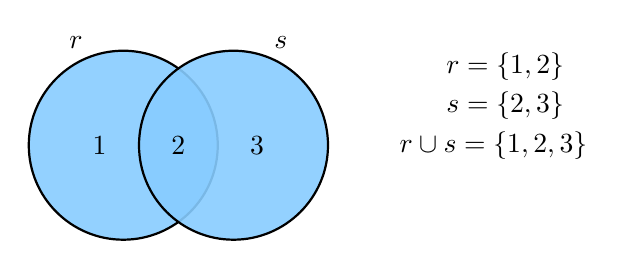
\begin{tikzpicture}[thick]
  \filldraw[fill=blue10, fill opacity=0.9]  (-0.7, 0.0) circle (1.2cm);
  \filldraw[fill=blue10, fill opacity=0.9]  ( 0.7, 0.0) circle (1.2cm); 
  \draw[color=black] (-1.0, 0.0) node {1};
  \draw[color=black] (0.0, 0.0) node {2};
  \draw[color=black] (1.0, 0.0) node {3};
  \draw[color=black] (-1.3, 1.3) node {$r$};
  \draw[color=black] (1.3, 1.3) node {$s$};
  \draw (4.15, 1.0)     node {$r = \{1,2\}$};
  \draw (4.15, 0.5)     node {$s = \{2,3\}$};  
  \draw (4.00, 0.0)     node {$r \cup s = \{1,2,3\}$};
\end{tikzpicture}
\pause
\begin{figure}[htp]
\en
\begin{tabular}[t]{ c c c }
  \begin{tabular}{ c c c } \toprule
    {\bf A} & {\bf B} & {\bf C}  \\ \midrule
    1 & b & 10 \\
    5 & a & 30 \\
    3 & c & 20 \\	\bottomrule
      &   &    \\
  \end{tabular} 
&  
  \begin{tabular}{ c c c }  \toprule
    {\bf A} & {\bf B} & {\bf C}  \\ \midrule
    5 & a & 30 \\
    2 & b & 10 \\
    3 & c & 20 \\	\bottomrule
      &   &    \\    
  \end{tabular} 
&  
  \begin{tabular}{ c c c }  \toprule
    {\bf A} & {\bf B} & {\bf C}  \\ \midrule
    1 & b & 10 \\
    5 & a & 30 \\
    3 & c & 20 \\
    2 & b & 10 \\	\bottomrule	
  \end{tabular}
\\  
  $r$ & $s$ & $r \cup s$ \\
\end{tabular}
\el
%\caption{\el Παράδειγμα σχεσιακής ένωσης: $t = r \cup s$}
\label{fig:ra_union_ex1}
\end{figure}
\end{minipage}
\end{frame}


\begin{frame}[t, fragile, shrink]
\frametitle{Ένωση και αντιμεταθετική ιδιότητα}
\begin{minipage}{\wE}
\begin{block}{Ισχύει η αντιμεταθετική ιδιότητα} \Large
    \[ r \cup s = s \cup r \]
\end{block}
\begin{exampleblock}{Παράδειγμα}
\en
\begin{tabular}{ c c c c }
  \begin{tabular}{ c c c } \toprule
    A & B & C \\ \midrule
    1 & b & 10 \\
    5 & a & 30 \\
    3 & c & 20 \\	\bottomrule
  \end{tabular} 
&  
  \begin{tabular}{ c c c }  \toprule
    {\bf A} & {\bf B} & {\bf C}  \\ \midrule
    5 & a & 30 \\
    2 & b & 10 \\
    3 & c & 20 \\	\bottomrule
  \end{tabular} 
&  
  \begin{tabular}{ c c c }  \toprule
    {\bf A} & {\bf B} & {\bf C}  \\ \midrule
    1 & b & 10 \\
    5 & a & 30 \\
    3 & c & 20 \\
    2 & b & 10 \\	\bottomrule	
  \end{tabular}
&  
  \begin{tabular}{ c c c }  \toprule
    {\bf A} & {\bf B} & {\bf C}  \\ \midrule
    5 & a & 30 \\
    2 & b & 10 \\
    3 & c & 20 \\  
    1 & b & 10 \\   \bottomrule	
  \end{tabular}  
\\  
  $r$ & $s$ & $r \cup s$ & $s \cup r$ \\
\end{tabular}
\el
\end{exampleblock}
\end{minipage}
\end{frame}



\begin{frame}[t, fragile, shrink]
\frametitle{Ένωση και προσεταιριστική ιδιότητα}
\begin{minipage}{\wE}
  \begin{block}{Ισχύει η προσεταιριστική ιδιότητα} \Large
    \[ r \cup (s \cup t) = (r \cup s) \cup t \]
  \end{block}
   Λόγω αυτής της της ιδιότητας, είναι δυνατό να γραφεί \\ η παρακάτω παράσταση χωρίς παρενθέσεις:
   \[
     r \cup s \cup t
   \]
   για να δηλώσει την ένωση τριών ή περισσότερων σχέσεων.
\end{minipage}
\end{frame}


\subsection[\textlatin{Difference}]{\textgreek{Η σχεσιακή πράξη της διαφοράς}}

\begin{frame}[t, fragile, shrink]
\frametitle{Η σχεσιακή πράξη της διαφοράς}
\begin{minipage}{\wE}
\large
\begin{block}{Ορισμός της διαφοράς:}
  \[
     r - s = \{t \,|\, t \in r \; \mathrm{and} \; t \notin s \}
  \]
  {\bb Διαφορά} δύο σχέσεων $r(R)$ και $s(S)$, που έχουν συμβατότητα τύπου, είναι μια νέα σχέση
  που έχει σχήμα (επικεφαλίδα) ίδιο με αυτό της $r$ και $s$, και κορμό 
  τις πλειάδες που ανήκουν στην $r$ αλλά όχι στην $s$.
  Η διαφορά συμβολίζεται με $r - s$  ή {\en $r \text{ MINUS }  s$}.
\end{block}
\end{minipage}
\end{frame}


\begin{frame}[t, fragile, shrink]
\frametitle{Παράδειγμα διαφοράς δύο σχέσεων}
\begin{minipage}{\wE}

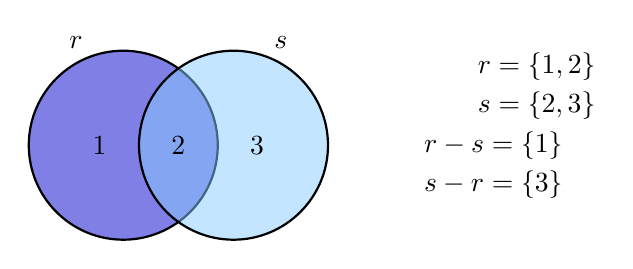
\begin{tikzpicture}[thick]
  \filldraw[fill=blue90, fill opacity=0.5]  (-0.7, 0.0) circle (1.2cm);
  \filldraw[fill=blue10, fill opacity=0.5]  ( 0.7, 0.0) circle (1.2cm); 
  \draw[color=black] (-1.0, 0.0) node {1};
  \draw[color=black] (0.0, 0.0) node {2};
  \draw[color=black] (1.0, 0.0) node {3};
  \draw[color=black] (-1.3, 1.3) node {$r$};
  \draw[color=black] (1.3, 1.3) node {$s$}; 
  \draw (4.55, 1.0)     node {$r = \{1,2\}$};
  \draw (4.55, 0.5)     node {$s = \{2,3\}$};  
  \draw (4.00, 0.0)     node {$r - s = \{1\}$};
  \draw (4.00,-0.5)     node {$s - r = \{3\}$};  
\end{tikzpicture}
\\
\pause
\par
\large
\en
\begin{tabular}{ c c c c }
  \begin{tabular}{ c c c } \toprule
    {\bf A} & {\bf B} & {\bf C}  \\ \midrule
    1 & b & 10 \\
    5 & a & 30 \\
    3 & c & 20 \\	\bottomrule
  \end{tabular} 
&  
  \begin{tabular}{ c c c }  \toprule
    {\bf A} & {\bf B} & {\bf C}  \\ \midrule
    5 & a & 30 \\
    2 & b & 10 \\
    3 & c & 20 \\	\bottomrule
  \end{tabular} 
&  
  \begin{tabular}{ c c c }  \toprule
    {\bf A} & {\bf B} & {\bf C}  \\ \midrule
    1 & b & 10 \\	\bottomrule
      &   &    \\
      &   &    \\
  \end{tabular}
&  
  \begin{tabular}{ c c c }  \toprule
    {\bf A} & {\bf B} & {\bf C}  \\ \midrule
    2 & b & 10 \\   \bottomrule
      &   &    \\
      &   &    \\    
  \end{tabular}  
\\  
  $r$ & $s$ & $r - s$ & $s - r$ \\
\end{tabular}
\el
\end{minipage}
\end{frame}


\begin{frame}[t, fragile, shrink]
\frametitle{Αντιμεταθετική και προσεταιριστική ιδιότητα}
\begin{minipage}{\wE}
  {\large Στη σχεσιακή πράξη της διαφοράς:}
  \begin{alertblock}{Δεν ισχύει η αντιμεταθετική ιδιότητα}
    \[ r - s \neq s - r \]
  \end{alertblock}
  \begin{alertblock}{Δεν ισχύει η προσεταιριστική ιδιότητα}
    \[ r - (s - t) \neq (r - s) - t \]
  \end{alertblock} 
  \begin{exampleblock}{Υπενθύμιση}
    \[ 5 - 3 \neq 3 - 5 \]
    \[ 8 - (3 - 2) \neq (8 - 3) - 2 \]
  \end{exampleblock}  
\end{minipage}
\end{frame}



\subsection[{\en Intersect}]{\textgreek{Η σχεσιακή πράξη της τομής}}


\begin{frame}[t, fragile, shrink]
\frametitle{Η σχεσιακή πράξη της τομής}
\begin{minipage}{\wE}
\large
\begin{block}{Ορισμός της τομής:}
  \[
     r \cap s = \{t \,|\, t \in r \; \mathrm{and} \; t \in s \}
  \]
  {\bb Τομή} δύο σχέσεων $r(R)$ και $s(S)$, που έχουν συμβατότητα τύπου,
  είναι μια νέα σχέση που έχει σχήμα (επικεφαλίδα) ίδιο με αυτό της $r$ και $s$,
  και κορμό τις πλειάδες που ανήκουν στην $r$ και στην $s$, δηλαδή τις κοινές πλειάδες.
  Η τομή συμβολίζεται με $r \cap s$  ή {\en $r  \text{ INTERSECT } s$}.
\end{block}
\end{minipage}
\end{frame}



\begin{frame}[t, fragile, shrink]
\frametitle{Παράδειγμα τομής δύο σχέσεων}
\begin{minipage}{\wE}

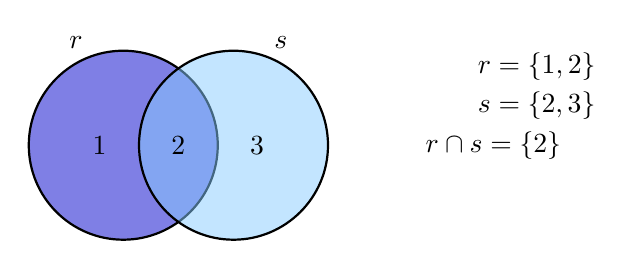
\begin{tikzpicture}[thick]
  \filldraw[fill=blue90, fill opacity=0.5]  (-0.7, 0.0) circle (1.2cm);
  \filldraw[fill=blue10, fill opacity=0.5]  ( 0.7, 0.0) circle (1.2cm); 
  \draw[color=black] (-1.0, 0.0) node {1};
  \draw[color=black] (0.0, 0.0) node {2};
  \draw[color=black] (1.0, 0.0) node {3};
  \draw[color=black] (-1.3, 1.3) node {$r$};
  \draw[color=black] (1.3, 1.3) node {$s$};
  \draw (4.55, 1.0)     node {$r = \{1,2\}$};
  \draw (4.55, 0.5)     node {$s = \{2,3\}$};  
  \draw (4.00, 0.0)     node {$r \cap s = \{2\}$};
\end{tikzpicture}
\\
\pause
\par
\large
\en
\begin{tabular}{ c c c }
  \begin{tabular}{ c c c } \toprule
    {\bf A} & {\bf B} & {\bf C} \\ \midrule
    1 & b & 10 \\
    5 & a & 30 \\
    3 & c & 20 \\   \bottomrule
  \end{tabular}
&
  \begin{tabular}{ c c c }  \toprule
    {\bf A} & {\bf B} & {\bf C} \\ \midrule
    5 & a & 30 \\
    2 & b & 10 \\
    3 & c & 20 \\   \bottomrule
  \end{tabular}
&
  \begin{tabular}{ c c c }  \toprule
    {\bf A} & {\bf B} & {\bf C}  \\ \midrule
    5 & a & 30 \\
    3 & c & 20 \\           \bottomrule
      &   &    \\
  \end{tabular}
\\
  $r$ & $s$ & $r \cap s$ \\
\end{tabular}
\el
\end{minipage}
\end{frame}


\begin{frame}[t, fragile, shrink]
\frametitle{Τομή και αντιμεταθετική ιδιότητα}
\begin{minipage}{\wE}
\begin{block}{Ισχύει η αντιμεταθετική ιδιότητα} \Large
    \[ r \cap s = s \cap r \]
\end{block}
\begin{exampleblock}{Παράδειγμα}
\en
\en
\begin{tabular}{ c c c c }
  \begin{tabular}{ c c c } \toprule
    {\bf A} & {\bf B} & {\bf C} \\ \midrule
    1 & b & 10 \\
    5 & a & 30 \\
    3 & c & 20 \\   \bottomrule
  \end{tabular}
&
  \begin{tabular}{ c c c }  \toprule
    {\bf A} & {\bf B} & {\bf C} \\ \midrule
    5 & a & 30 \\
    2 & b & 10 \\
    3 & c & 20 \\   \bottomrule
  \end{tabular}
&
  \begin{tabular}{ c c c }  \toprule
    {\bf A} & {\bf B} & {\bf C}  \\ \midrule
    5 & a & 30 \\
    3 & c & 20 \\           \bottomrule
      &   &    \\
  \end{tabular}
&
  \begin{tabular}{ c c c }  \toprule
    {\bf A} & {\bf B} & {\bf C}  \\ \midrule
    5 & a & 30 \\
    3 & c & 20 \\           \bottomrule
      &   &    \\    
  \end{tabular}
\\
  $r$ & $s$ & $r \cap s$ & $s \cap r$ \\
\end{tabular}
\el
\el
\end{exampleblock}
\end{minipage}
\end{frame}


\begin{frame}[t, fragile, shrink]
\frametitle{Τομή και προσεταιριστική ιδιότητα}
\begin{minipage}{\wE}
  \begin{block}{Ισχύει η προσεταιριστική ιδιότητα} \Large
    \[ r \cap (s \cap t) = (r \cap s) \cap t \]
  \end{block}
   Λόγω αυτής της της ιδιότητας, είναι δυνατό να γραφεί \\ η παρακάτω παράσταση χωρίς παρενθέσεις:
   \[
     r \cap s \cap t
   \]
   για να δηλώσει την τομή τριών ή περισσότερων σχέσεων.
\end{minipage}
\end{frame}


\begin{frame}[t, fragile, shrink]
\frametitle{Η τομή είναι παράγωγη πράξη}
\begin{minipage}{\wE}
  \begin{block}{Εναλλακτικός ορισμός της τομής} \Large
    \[
       r \cap s = r - (r-s)
    \]
  \end{block}
   Δηλαδή το αποτέλεσμα της τομής $r \cap s$ ισούται με το αποτέλεσμα της διαφοράς
   της $r$ από τη διαφορά $r-s$.
   \begin{exampleblock}{Παράδειγμα}
     Δώστε εσείς ένα παράδειγμα που να επιβεβαιώνει (ή να αναιρεί)
     τον παραπάνω ορισμό.
   \end{exampleblock}
\end{minipage}
\end{frame}


\subsection[{\en Examples}]{\textgreek{Επιπλέον παραδείγματα συνολοθεωρητικών πράξεων}}

\begin{frame}[t, fragile, shrink]
\frametitle{\en Pane Amore}
\begin{minipage}{\wE}
  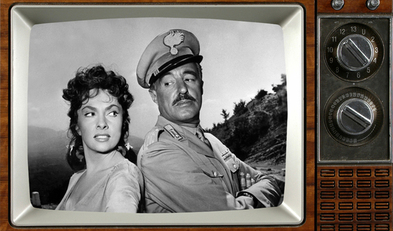
\includegraphics[scale=0.65]{pane-amore.jpg} \\
  \en
  \begin{enumerate}
    \item Pane, amore e fantasia, (1953)
    \item Pane, amore e gelosia, (1954)
    \item Pane, amore e ..., (1955)
  \end{enumerate}
\end{minipage}
\end{frame}

\begin{frame}[t, fragile, shrink]
\frametitle{\en Pane amore}
\begin{minipage}{\wE}
\en
\begin{tabular}{ c c }
  $f$ & $g$ \\
  \begin{tabular}{ c l }              \toprule
    {\bf actorID}  &  {\bf name} \\   \midrule
    0001120  &   Vittorio De Sica \\
    0518178  &   Gina Lollobrigida \\
    0581028  &   Marisa Merlini \\
    0139214  &   Memmo Carotenuto \\
    0728376  &   Roberto Risso \\
    0681365  &   Tina Pica \\
    0188022  &   Vittoria Crispo \\   \bottomrule
  \end{tabular}
  &
  \begin{tabular}{ c l }              \toprule
    {\bf actorID}  &  {\bf name} \\   \midrule
    0001120  &   Vittorio De Sica \\
    0518178  &   Gina Lollobrigida \\
    0581028  &   Marisa Merlini \\
    0139214  &   Memmo Carotenuto \\
    0681365  &   Tina Pica \\
    0882237  &   Saro Urzì \\
    0188022  &   Vittoria Crispo \\     \bottomrule
  \end{tabular}
  \\
\end{tabular}
\el
\end{minipage}
\end{frame}


\begin{frame}[t, fragile, shrink]
\frametitle{{\en Pane amore} (Ερωτήματα συμμετοχής) }
\begin{minipage}{\wE}
  \begin{block}{Έπαιξαν σε τουλάχιστον μία ταινία}
    \[ f \cup g \]
  \end{block}
  \begin{block}{Έπαιξαν και στις δύο πρώτες ταινίες}
    \[ f \cap g \]
  \end{block}
  \begin{block}{Έπαιξαν μόνο στην πρώτη ταινία}
    \[ f - g \]
  \end{block}
  \begin{block}{Έπαιξαν μόνο στη δεύτερη ταινία}
    \[ g - f  \]
  \end{block}
\end{minipage}
\end{frame}



\begin{frame}[t, fragile, shrink]
\frametitle{Τομή {\en fantasia $\cap$ gelosia}}
\begin{minipage}{\wE}
\en
\scriptsize
\begin{tabular}{ c c }
  $f$ & $g$ \\
  \begin{tabular}{ c l }              \toprule
    {\bf actorID}  &  {\bf name} \\   \midrule
    0001120  &   Vittorio De Sica \\
    0518178  &   Gina Lollobrigida \\
    0581028  &   Marisa Merlini \\
    0139214  &   Memmo Carotenuto \\
    0728376  &   Roberto Risso \\
    0681365  &   Tina Pica \\
    0188022  &   Vittoria Crispo \\   \bottomrule
  \end{tabular}
  &
  \begin{tabular}{ c l }              \toprule
    {\bf actorID}  &  {\bf name} \\   \midrule
    0001120  &   Vittorio De Sica \\
    0518178  &   Gina Lollobrigida \\
    0581028  &   Marisa Merlini \\
    0139214  &   Memmo Carotenuto \\
    0681365  &   Tina Pica \\
    0882237  &   Saro Urzì \\
    0188022  &   Vittoria Crispo \\     \bottomrule
  \end{tabular}
  \\
\end{tabular}
\normalsize  \color{blue}
  \begin{tabular}{ c l }              \toprule
    {\bf actorID}  &  {\bf name} \\              \midrule
    0001120  &   Vittorio De Sica \\
    0518178  &   Gina Lollobrigida \\
    0581028  &   Marisa Merlini \\
    0139214  &   Memmo Carotenuto \\ 
    0681365  &   Tina Pica \\     
    0188022  &   Vittoria Crispo \\  \bottomrule
  \end{tabular}
\el
\end{minipage}
\end{frame}


\begin{frame}[t, fragile, shrink]
\frametitle{Διαφορά {\en fantasia $-$ gelosia}}
\begin{minipage}{\wE}
\en
\scriptsize
\begin{tabular}{ c c }
  $f$ & $g$ \\
  \begin{tabular}{ c l }              \toprule
    {\bf actorID}  &  {\bf name} \\   \midrule
    0001120  &   Vittorio De Sica \\
    0518178  &   Gina Lollobrigida \\
    0581028  &   Marisa Merlini \\
    0139214  &   Memmo Carotenuto \\
    0728376  &   Roberto Risso \\
    0681365  &   Tina Pica \\
    0188022  &   Vittoria Crispo \\   \bottomrule
  \end{tabular}
  &
  \begin{tabular}{ c l }              \toprule
    {\bf actorID}  &  {\bf name} \\   \midrule
    0001120  &   Vittorio De Sica \\
    0518178  &   Gina Lollobrigida \\
    0581028  &   Marisa Merlini \\
    0139214  &   Memmo Carotenuto \\
    0681365  &   Tina Pica \\
    0882237  &   Saro Urzì \\
    0188022  &   Vittoria Crispo \\     \bottomrule
  \end{tabular}
  \\
\end{tabular}
\bigskip
\normalsize      \color{blue}
  \begin{tabular}{ c l }              \toprule
    {\bf actorID}  &  {\bf name} \\              \midrule
    0728376  &   Roberto Risso \\  \bottomrule
  \end{tabular}
\el
\end{minipage}
\end{frame}




%\maketitle

\section[{\en Cartesian Product}]{\textgreek{Η σχεσιακή πράξη του γινομένου}}
\subsection[{\en Cartesian Product}]{\textgreek{Το καρτεσιανό γινόμενο και οι εφαρμογές του}}

\begin{frame}[t, fragile, shrink]
\frametitle{Η σχεσιακή πράξη του γινομένου}
\begin{minipage}{\wE}
  \begin{block}{Ορισμός του γινομένου} \en \Large
    \[
       r \times s = \{ t \, u \, | \, t \in r \text{ and }  u \in s\}
    \]
    \el
    \large
    {\bb Καρτεσιανό γινόμενο} δύο σχέσεων $r(R)$ και $s(S)$,
    είναι μια σχέση που έχει επικεφαλίδα το σύνολο των γνωρισμάτων των σχέσεων $R$ και $S$,
    και κορμό το σύνολο όλων των συνδυασμών
    των πλειάδων που ανήκουν στην $r$ και στην $s$.
    Το καρτεσιανό γινόμενο συμβολίζεται με $r \times s$  ή {\en $r \text{ TIMES } s$}.
  \end{block}
\end{minipage}
\end{frame}


\begin{frame}[t, fragile, shrink]
\frametitle{Γνωρίσματα καρτεσιανού γινομένου}
\begin{minipage}{\wE}
  \begin{block}{Μετονομασία κοινών γνωρισμάτων}
    Το σχήμα ενός καρτεσιανού γινομένου προκύπτει μετά από μετονομασία
    των πιθανών κοινών γνωρισμάτων δύο σχέσεων. \\
    Για παράδειγμα, αν $Y$ είναι ένα κοινό γνώρισμα των σχέσεων $r(R)$ και $s(S)$,
    τότε το σχήμα της σχέσης $r \times s$ είναι:
    \par
    \large
    \[
       T = (R-S) \cup (S-R) \cup \{R.Y , S.Y \,|\, Y \in R \cap S\}
    \]
  \end{block}
\end{minipage}
\end{frame}


\begin{frame}[t, fragile, shrink]
\frametitle{Βαθμός και πληθικότητα γινομένου}
\begin{minipage}{\wE}
  \begin{block}{Βαθμός γινομένου}
    Αν η σχέση $r$ είναι $n_R$ βαθμού
    και η σχέση $s$ είναι $n_S$ βαθμού τότε το αποτέλεσμα του γινομένου έχει βαθμό:
    \[
       n_{r \times s}  = n_R + n_S
    \]
  \end{block}
  \begin{block}{Πληθικότητα γινομένου}
    Αν η σχέση $r$ είναι $m_r$ βαθμού
    και η σχέση $s$ είναι $m_s$ βαθμού τότε το αποτέλεσμα του γινομένου έχει βαθμό:
    \[
       m_{r \times s}  =m_r \cdot m_s
    \]
  \end{block}
\end{minipage}
\end{frame}



\begin{frame}[t, fragile, shrink]
\frametitle{Παράδειγμα σχεσιακού γινομένου}
\begin{minipage}{\wE}
  %\begin{block}{}
\en
\begin{tabular}{ c c c }
  $r$ & $s$ & $r \times s$ \\
  \begin{tabular}{ c c } \toprule
    {\bf A} & {\bf B}  \\            \midrule
    1 & b  \\
    5 & a  \\
    3 & c  \\            \bottomrule
      &    \\
      &    \\
      &    \\
  \end{tabular}
&
  \begin{tabular}{ c c c }  \toprule
    {\bf D} & {\bf E} & {\bf F} \\ \midrule
    b & 4 & 30 \\
    a & 2 & 10 \\ \bottomrule
      &    \\
      &    \\
      &    \\
      &    \\
  \end{tabular}
&
  \begin{tabular}{ c c c c c }  \toprule
    {\bf A} & {\bf B} & {\bf D} & {\bf E} & {\bf F}  \\ \midrule
    1 & b & b & 4 & 30 \\
    1 & b & a & 2 & 10 \\
    5 & a & b & 4 & 30 \\
    5 & a & a & 2 & 10 \\
    3 & c & b & 4 & 30 \\
    3 & c & a & 2 & 10 \\    \bottomrule
  \end{tabular}
\\
\end{tabular}
\el
  %\end{block}
\end{minipage}
\end{frame}



\begin{frame}[t, fragile, shrink]
\frametitle{Γινόμενο και μετονομασία γνωρισμάτων}
\begin{minipage}{\wE}
\en
\begin{tabular}{ c c c }
  $r$ & $s$ & $r \times s$ \\
  \begin{tabular}{ c c } \toprule
    {\bf A} & {\bf B}  \\            \midrule
    1 & b  \\
    5 & a  \\
    3 & c  \\            \bottomrule
      &    \\
      &    \\
      &    \\
  \end{tabular}
&
  \begin{tabular}{ c c c }  \toprule
    {\bf A} & {\bf B} & {\bf F} \\ \midrule
    b & 4 & 30 \\
    a & 2 & 10 \\ \bottomrule
      &    \\
      &    \\
      &    \\
      &    \\
  \end{tabular}
&
  \begin{tabular}{ c c c c c }  \toprule
    {\bf R.A} & {\bf R.B} & {\bf S.A} & {\bf S.B} & {\bf F}  \\ \midrule
    1 & b & b & 4 & 30 \\
    1 & b & a & 2 & 10 \\
    5 & a & b & 4 & 30 \\
    5 & a & a & 2 & 10 \\
    3 & c & b & 4 & 30 \\
    3 & c & a & 2 & 10 \\    \bottomrule
  \end{tabular}
\\
\end{tabular}
\el
\end{minipage}
\end{frame}


\begin{comment}
\begin{frame}
\frametitle{Ιδιότητες του γινομένου}
\begin{block}{Αντιμεταθετική ιδιότητα}
\[
r \times s = s \times r
\]
Δηλαδή δεν έχει σημασία η σειρά των τελεσταίων, με οποιαδήποτε σειρά και να γίνει η πράξη
της τομής το αποτέλεσμα είναι το ίδιο.
\end{block}
\begin{block}{Προσεταιριστική ιδιότητα}
\[
r \times (s \times t) = (r \times s) \times t
\]
\end{block}
\end{frame}

\begin{frame}
\frametitle{Παράδειγμα γινομένου με σύνολα}
Αν
\[ A=\{a,b,c\} \]
και \[ B=\{1,2\}\]
τότε
\[
Α \times B = \{(a,1), (a,2), (b,1), (b,2), (c,1), (c,2) \}
\]
Δηλαδή το γινόμενο δύο συνόλων $A$ και $B$ αποτελείται από όλους
τους συνδυασμούς των μελών των $A$ και $B$.
\end{frame}
\end{comment}


\begin{frame}[t, fragile, shrink]
\frametitle{Δενδροειδής απεικόνιση καρτεσιανού γινομένου}
\begin{minipage}{\wE}
  \begin{columns}[T]
    \begin{column}{0.5\textwidth}
      \en
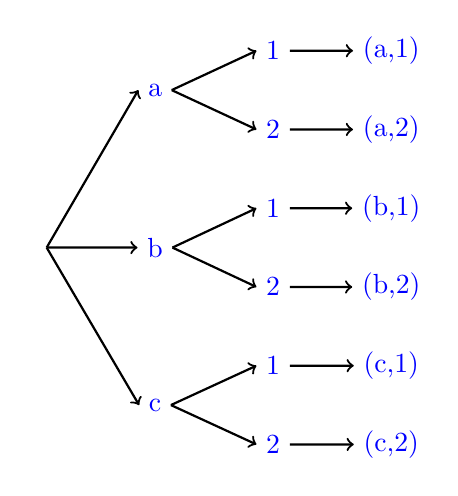
\begin{tikzpicture}
  [parent anchor=east,child anchor=west, grow=east, 
  every node/.style={circle,draw},  
  level 1/.style={sibling distance=20mm},
  level 2/.style={sibling distance=10mm},
  level 3/.style={sibling distance=10mm},
 ]
  \tikzstyle{every node}=[text=blue]
  \tikzstyle{edge from parent}=[draw, ->, solid, thick, black]
\node { }
  child {node {c} 
    child {node {2} child {node {(c,2)}} }
    child {node {1} child {node {(c,1)}} }
  }
  child {node {b} 
    child {node {2} child {node {(b,2)}} }
    child {node {1} child {node {(b,1)}} }
  }
  child {node {a}
    child {node {2} child {node {(a,2)}} }
    child {node {1} child {node {(a,1)}} }
  };
\end{tikzpicture}
\el

    \end{column}
    \begin{column}{0.5\textwidth}
     \begin{align*}
       A &=& \{a,b,c\} \\
       B &=& \{1,2\}  \\
       A \times B &=& \{ (a,1), (a,2) \\
                  &&     (b,1), (b,2), \\
                  &&     (c,1), (c,2) \}
     \end{align*}
    \end{column}
  \end{columns}
\end{minipage}
\end{frame}


\begin{frame}[t, fragile, shrink]
\frametitle{Απεικόνιση καρτεσιανού γινομένου σε σύνολα}
\begin{minipage}{\wE}
  \begin{columns}[T]
    \begin{column}{0.5\textwidth}
      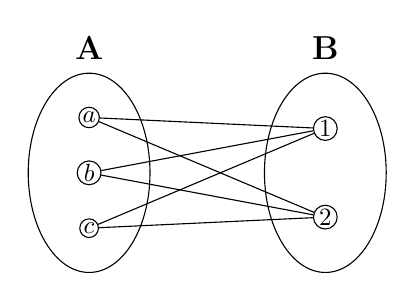
\begin{tikzpicture}
  \tikzstyle{every state} = [fill, draw=black, blue50, text=black]
  \tikzstyle{every state} = [inner sep=0.5pt, minimum size=0pt, scale=0.9]
   
  \def\A{0.0};
  \def\B{3.0};

  \draw (\A, 0) ellipse (22pt and 36pt); % A
  \draw (\B, 0) ellipse (22pt and 36pt); % B

  % A nodes
  \node[state] (a1) at (\A,  20pt) {$a$};
  \node[state] (a2) at (\A,   0pt) {$b$};
  \node[state] (a3) at (\A, -20pt) {$c$};

  % B nodes
  \node[state] (b1) at (\B,  16pt) {$1$};
  \node[state] (b2) at (\B, -16pt) {$2$};

  % connection lines
  \path[-] (a1) edge  (b1);
  \path[-] (a2) edge  (b1);
  \path[-] (a3) edge  (b1);
  \path[-] (a1) edge  (b2);
  \path[-] (a2) edge  (b2);
  \path[-] (a3) edge  (b2);
  

  % annotate names
  \draw (\A, 45pt) node {\large$\mathbf{A}$};
  \draw (\B, 45pt) node {\large$\mathbf{B}$};

\end{tikzpicture}

    \end{column}
    \begin{column}{0.5\textwidth}
     \begin{align*}
       A &=& \{a,b,c\} \\
       B &=& \{1,2\}  \\
       A \times B &=& \{ (a,1), (a,2) \\
                  &&     (b,1), (b,2), \\
                  &&     (c,1), (c,2) \}
     \end{align*}
    \end{column}
  \end{columns}
\end{minipage}
\end{frame}



\begin{frame}[t, fragile, shrink]
\frametitle{Προσοχή στο καρτεσιανό γινόμενο}
\begin{minipage}{\wE}
  \begin{exampleblock}{Φοιτητές και Μαθήματα}
    Αν $M$ είναι το σύνολο των μαθημάτων 
    και $\Phi$ είναι το σύνολο των φοιτητών 
    τότε
    \vspace*{-0.5cm} \[ M \times \Phi \]    %\vspace*{-0.5cm}
    είναι ο συνδυασμός όλων των μαθημάτων με όλους τους φοιτητές
    (όλοι εξετάζονται σε όλα).
  \end{exampleblock}
  \begin{exampleblock}{Ηθοποιοί και ταινίες}
    Αν $H$ είναι το σύνολο των ηθοποιών
    και $T$ είναι το σύνολο των ταινιών
    τότε \vspace*{-0.5cm}    \[ H \times T \]    %\vspace*{-0.5cm}
    είναι ο συνδυασμός όλων των ηθοποιών με όλες τις ταινίες
    (όλοι παίζουν σε όλες).
  \end{exampleblock}

\end{minipage}
\end{frame}


%\maketitle

\section[{\en join}]{\textgreek{Σύζευξη και είδη συζεύξεων}}

\subsection[{\en natjoin}]{\textgreek{Φυσική σύζευξη}}

\begin{frame}[t, fragile, shrink]
\frametitle{Η σχεσιακή πράξη της φυσικής σύζευξης}
\begin{minipage}{\wE}
  \begin{block}{Ορισμός της φυσικής σύζευξης} 
    \[
       \begin{split}
       r \bowtie s = \{ t \,|\, \text{ υπάρχουν πλειάδες } \, u \in r \text{ και } v \in s   \\
                \text{ έτσι ώστε } t[R]=u \text{ και } t[S]=v\}         
       \end{split}
    \]
    \par Αν η $r$ είναι σχέση με σχήμα $R=\{X,Y\}$ και $s$ είναι σχέση με σχήμα $S=\{Y,Z\}$,
    τότε η {\bf φυσική σύζευξη} των $r$ και $s$
    είναι μια σχέση με σχήμα $R \cup S = \{X,Y,Z\}$ και κορμό το σύνολο των συνδυασμών των
    πλειάδων της $r$ και $s$ για τις οποίες οι τιμές στο κοινό γνώρισμα $Y$ ταυτίζονται.   \\
    Η φυσική σύζευξη των σχέσεων $r$ και $s$ συμβολίζεται με $r \bowtie s$,
    ή $r \, \mathrm{NATURAL\, JOIN} \, s$, ή απλά $r \, \mathrm{JOIN} \, s$.
  \end{block}
\end{minipage}
\end{frame}



\begin{frame}[t, fragile, shrink]
\frametitle{Παράδειγμα φυσικής σύζευξης}
  \scalebox{1.5}{ \en
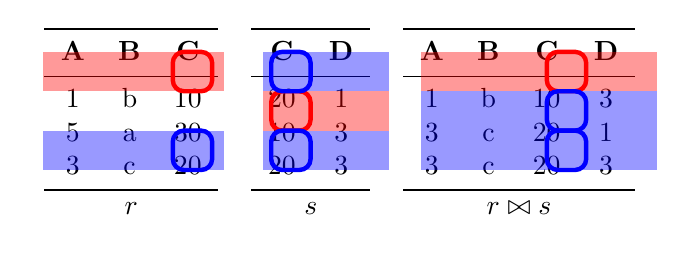
\begin{tikzpicture}

\node[anchor=south west,inner sep=0] at (0,0)
{
\begin{tabular}{ c c c }
  \begin{tabular}{ c c c }    \toprule
    {\bf A} & {\bf B} & {\bf C}  \\             \midrule
    1 & b & 10 \\
    5 & a & 30 \\
    3 & c & 20 \\             \bottomrule
  \end{tabular}
&
  \begin{tabular}{ c c }      \toprule
    {\bf C} & {\bf D}   \\                \midrule
    20 & 1  \\
    10 & 3  \\
    20 & 3  \\                \bottomrule
  \end{tabular}
&
  \begin{tabular}{ c c c c }  \toprule
    {\bf A} & {\bf B} & {\bf C}  & {\bf D}  \\        \midrule
    1 & b & 10 & 3  \\
    3 & c & 20 & 1  \\
    3 & c & 20 & 3  \\        \bottomrule
  \end{tabular}
\\
  $r$ & $s$ & $r \bowtie s$ \\
\end{tabular}  
} ;


% red 10
\pause
\draw[red,ultra thick,rounded corners] (1.85,1.7) rectangle node[above] {} + (0.5,0.5);
\draw[red,ultra thick,rounded corners] (3.10,1.2) rectangle node[above] {} + (0.5,0.5);

% red rows
\pause
\draw[red,ultra thick,rounded corners] (6.60,1.7) rectangle node[above] {} + (0.5,0.5);
\fill[red, opacity=0.4]      (0.20,1.7) rectangle node[above] {} + (2.3,0.5);
\fill[red, opacity=0.4]      (3.00,1.2) rectangle node[above] {} + (1.6,0.5);
\fill[red, opacity=0.4]      (5.00,1.7) rectangle node[above] {} + (3.0,0.5);

% blue 20
\pause
\draw[blue,ultra thick,rounded corners] (1.85,0.7) rectangle node[above] {} + (0.5,0.5);
\draw[blue,ultra thick,rounded corners] (3.10,1.7) rectangle node[above] {} + (0.5,0.5);
\draw[blue,ultra thick,rounded corners] (3.10,0.7) rectangle node[above] {} + (0.5,0.5);

%blue rows 
\pause
\draw[blue,ultra thick,rounded corners] (6.60,1.2) rectangle node[above] {} + (0.5,0.5);
\draw[blue,ultra thick,rounded corners] (6.60,0.7) rectangle node[above] {} + (0.5,0.5);
\fill[blue, opacity=0.4]      (0.20,0.7) rectangle node[above] {} + (2.3,0.5);
\fill[blue, opacity=0.4]      (3.00,1.7) rectangle node[above] {} + (1.6,0.5);
\fill[blue, opacity=0.4]      (3.00,0.7) rectangle node[above] {} + (1.6,0.5);
\fill[blue, opacity=0.4]      (5.00,1.2) rectangle node[above] {} + (3.0,0.5);
\fill[blue, opacity=0.4]      (5.00,0.7) rectangle node[above] {} + (3.0,0.5);


\end{tikzpicture}
\el  } 
  \begin{minipage}{\wE} 
    \begin{block}{Παρατηρήσεις}
      \begin{enumerate}
        \item Τα κοινά γνωρίσματα, εδώ το {\en\em C}, μόνο μία φορά στο αποτέλεσμα.
        \item Πλειάδες με μη ταιριαστές τιμές δεν συμμετέχουν στο αποτέλεσμα.
      \end{enumerate}
  \end{block}
\end{minipage}
\end{frame}

\begin{frame}[t, fragile, shrink]
\frametitle{Υπάλληλοι και τμήματα, ξένο κλειδί, 1:Ν}
\small
%\begin{minipage}{\wE}
  \begin{tabular} { l  l }
    \shortstack{
    {\bb\en departments}: \\ 
    \begin{tabular}{ c l } \toprule
    {\en\bf depid} & {\en\bf depname} \\ \midrule
    1 & Μελετών \\
    2 & Λογιστήριο \\
    3 & Διαφήμισης \\ \bottomrule
      & \\
      & \\ 
    \end{tabular}
    }
    &
    \shortstack{
    {\bb\en employees}: \\  
    \begin{tabular}{ c l c } \toprule
      {\en\bf empid} & {\en\bf empname} & {\en\bf depid} \\ \midrule
      102 & Αποστολάκης & 2 \\
      154 & Βασιλάκης   & 1 \\
      132 & Χρηστάκης   & 2\\ 
      432 & Δημητράκης  & 3 \\
      203 & Κωστάκης    & 1 \\ \bottomrule
    \end{tabular}
    }
  \end{tabular}
  \par
  %\bigskip
  {\bb\en departments $\bowtie$ employees}: \\
  \begin{tabular}{ c l c l } \toprule
    {\en\bf depid} & {\en\bf depname} & {\en\bf empid} & {\en\bf empname} \\ \midrule
    1 & Μελετών & 154 & Βασιλάκης  \\
    1 & Μελετών & 203 & Κωστάκης   \\
    2 & Λογιστήριο & 102 & Αποστολάκης \\
    2 & Λογιστήριο & 132 & Χρηστάκης \\
    3 & Διαφήμισης & 432 & Δημητράκης \\ \bottomrule
  \end{tabular} 

%\end{minipage}
\end{frame}


\subsection[{\en theta}]{\textgreek{Θήτα σύζευξη}}


\begin{frame}[t, fragile, shrink]
\frametitle{Η σχεσιακή πράξη της σύζευξης θ}
\begin{minipage}{\wE}
  \begin{block}{Ορισμός}
    \par Αν η $r$ είναι σχέση με σχήμα $R=\{A_1, A_2, \ldots, A_n\}$,
    $s$ είναι σχέση
    με σχήμα $S=\{B_1, B_2, \ldots, B_m\}$,
    τα γνωρίσματα $A_i$ και $B_j$ έχουν το ίδιο πεδίο ορισμού,
    και $\theta$ είναι τελεστής σύγκρισης, $\theta \in \{=,\neq,<,\leq,>,\geq\}$, 
    \par τότε η $\theta$ σύζευξη των $r$ και $s$, $r \bowtie_{A_i \theta B_j} s$,
    \par είναι μια σχέση με σχήμα
    το σύνολο των γνωρισμάτων των $R$ και $S$, $\{A_1, A_2, \ldots, A_n\, B_1, B_2, \ldots, B_m\}$
    και κορμό το σύνολο των πλειάδων από κάθε συνδυασμό των πλειάδων των $r$ και $s$,
    που ικανοποιούν τη συνθήκη $A_i \theta B_j$.
  \end{block}
\end{minipage}
\end{frame}



\begin{frame}[t, fragile, shrink]
\frametitle{Παρατηρήσεις για τη θ σύζευξη}
\begin{minipage}{\wE}
  \begin{itemize}   \itemsep6pt
    \item Το αποτέλεσμα είναι μια σχέση με βαθμό $n_R+n_S$,
          και πληθικότητα ανάμεσα στο 0 και στο $m_r \cdot m_s$.
    \item Αν κάποια πλειάδα έχει στο γνώρισμα που συμμετέχει
          στη σύζευξη  τιμή {\sq NULL} τότε δεν συμμετέχει στο αποτέλεσμα.
    \item Αν ο τελεστής $\theta$ είναι το $=$ τότε η σύζευξη καλείται {\bb ισοσύζευξη}.
    \item Η σύζευξη $\theta$ ($\theta\, \mathrm{JOIN}$) είναι παράγωγη πράξη γινομένου και επιλογής,
          έτσι ισχύει: \\
          {\Large \[ \sigma_{X \theta Y}(r \times s) = r \bowtie_{X \theta Y} s \]  }
  \end{itemize}
\end{minipage}
\end{frame}



\begin{frame}[t, fragile, shrink]
\frametitle{Παράδειγμα  σύζευξης θ, ξένο κλειδί, 1:Ν }
  \vspace{-1em}
  \begin{columns}[T]
    \begin{column}{0.5\textwidth}
    {\bb\en departments}:\\
    \begin{tabular}{c l} \toprule
      {\en\bf depcode} & {\en\bf depname} \\ \midrule
      1 & Μελετών \\
      2 & Λογιστήριο \\
      3 & Διαφήμισης \\ \bottomrule
    \end{tabular}
    \end{column}
    \begin{column}{0.5\textwidth}
    {\bb\en employees}: \\
    \begin{tabular}{c l c} \toprule
      {\en\bf empid} & {\en\bf empname} & {\en\bf depid} \\ \midrule
      102 & Αποστολάκης & 2 \\
      154 & Βασιλάκης   & 1 \\
      132 & Χρηστάκης   & 2\\
      432 & Δημητράκης  & 3 \\
      203 & Κωστάκης    & 1 \\ \bottomrule
    \end{tabular} 
    \end{column}
  \end{columns}
  \par
  \bigskip
  {\bb\en departments $\bowtie_{depcode=depid}$ employees}: \\
  \begin{tabular}{c l c l c} \toprule
    {\en\bf depcode} & {\en\bf depname} & {\en\bf empid} & {\en\bf empname} & {\en\bf depid} \\ \midrule
    1 & Μελετών & 154 & Βασιλάκης  & 1\\
    1 & Μελετών & 203 & Κωστάκης   & 1\\
    2 & Λογιστήριο & 102 & Αποστολάκης & 2\\
    2 & Λογιστήριο & 132 & Χρηστάκης  & 2\\
    3 & Διαφήμισης & 432 & Δημητράκης & 3\\ \\bottomrule
  \end{tabular}
\end{frame}



\begin{frame}[t, fragile, shrink]
\frametitle{Ενδυματολογικές προτιμήσεις και θ σύζευξη}
\begin{minipage}{\wE}
  %\begin{block}{Παπούτσια και Φούστες}
    \en
    \begin{columns}[T]
      \begin{column}{0.5\textwidth}
        {\bb\en shoes:} \\
        \begin{tabular}{l c}  \toprule
          {\en\bf color} & {\en\bf price} \\     \midrule
          blue  & 55 \\
          green & 45 \\
          red   & 30 \\ \bottomrule
                &    \\
        \end{tabular}
      \end{column}
      \begin{column}{0.5\textwidth}
        {\bb\en skirts:} \\
        \begin{tabular}{l c}  \toprule
          {\en\bf color} & {\en\bf price} \\     \midrule
          red     & 30 \\
          green   & 40 \\
          green   & 65 \\
          blue    & 30 \\ \bottomrule
        \end{tabular}
      \end{column}
    \end{columns}
    \el
  %\end{block}
  \begin{block}{Να βρεθούν οι συνδυασμοί:}
    \begin{enumerate}  \itemsep9pt
      \item Παπούτσια και φούστες ίδιου χρώματος.
      \item Παπούτσια και φούστες διαφορετικού χρώματος.
      \item Παπούτσια και φούστες με ακριβότερη τη φούστα.
    \end{enumerate}
  \end{block}
\end{minipage}
\end{frame}


\begin{frame}[t, fragile, shrink]
\frametitle{Παπούτσια και φούστες ίδιου χρώματος}
\begin{minipage}{\wE}
  {\Large \[ shoes \bowtie_{shoes.color=skirts.color} skirts \]  }
  \par
  \en
  \begin{tabular}{l c l c}  \toprule
    {\en\bf shoes.color} & {\en\bf shoes.price} & {\en\bf skirts.color} & {\en\bf skirts.price}\\     \midrule
       blue  & 55 & blue & 30 \\
       green & 45 & green & 40 \\
       green & 45 & green & 65 \\
       red   & 30 & red & 30 \\ \bottomrule
  \end{tabular}
\end{minipage}
\end{frame}


\begin{frame}[t, fragile, shrink]
\frametitle{Παπούτσια και φούστες διαφορετικού χρώματος}
\begin{minipage}{\wE}
  {\Large \[ shoes \bowtie_{shoes.color \neq skirts.color} skirts \]  }
  \par
  \en
  \begin{tabular}{l c l c}  \toprule
    {\en\bf shoes.color} & {\en\bf shoes.price} & {\en\bf skirts.color} & {\en\bf skirts.price}\\     \midrule
       blue  & 55 & red   & 30 \\
       blue  & 55 & green & 40 \\
       blue  & 55 & green & 65 \\
       green & 45 & red   & 30 \\
       green & 45 & blue  & 30 \\
       red   & 30 & green & 40 \\
       red   & 30 & green & 65 \\
       red   & 30 & blue  & 30 \\ \bottomrule
  \end{tabular}
\end{minipage}
\end{frame}


\begin{frame}[t, fragile, shrink]
\frametitle{Παπούτσια και φούστες με ακριβότερη φούστα}
\begin{minipage}{\wE}
  {\Large \[ shoes \bowtie_{shoes.price < skirts.price} skirts \]  }
  \par
  \en
  \begin{tabular}{l c l c}  \toprule
    {\en\bf shoes.color} & {\en\bf shoes.price} & {\en\bf skirts.color} & {\en\bf skirts.price}\\     \midrule
       blue  & 55 & green & 65 \\
       green & 45 & green & 65 \\
       red   & 30 & green & 40 \\
       red   & 30 & green & 65 \\ \bottomrule
  \end{tabular}
\end{minipage}
\end{frame}


\subsection[{\en outerjoin}]{\textgreek{Εξωτερική σύζευξη}}


\begin{frame}[t, fragile, shrink]
\frametitle{Eξωτερική σύζευξη}
\begin{minipage}{\wE}
\begin{block}{Ορισμός εξωτερική σύζευξης}
  Αν η $r$ είναι σχέση με σχήμα $R= \{ X, Y \} $,
  $s$ είναι σχέση με σχήμα $S=\{Y, Z\}$,
  τότε η εξωτερική σύζευξη
  $t = r \ojoin s$ έχει σχήμα $T=\{X,Y,Z\}$ και κορμό που
  αποτελείται από : 
  \vspace{0.5cm}
  \begin{enumerate} \itemsep 6pt
    \item Τις πλειάδες της εσωτερικής σύζευξης  των $r \bowtie s$
    \item Τις πλειάδες της σχέσης $r$ που δεν έχουν ταιριαστές τιμές στην $s$,
          με τιμές {\sq NULL} στα αντίστοιχα γνωρίσματα της $s$
    \item Τις πλειάδες της σχέσης $s$ που δεν έχουν ταιριαστές τιμές στην $r$,
          με τιμές {\sq NULL} στα αντίστοιχα γνωρίσματα της $r$
  \end{enumerate}
\end{block}
\end{minipage}
\end{frame}


\begin{frame}[t, fragile, shrink]
\frametitle{Εξωτερική σύζευξη}
  \begin{block}{Επέκταση της σύζευξης}
    Η εξωτερική σύζευξη είναι επέκταση της σύζευξης, στην περίπτωση που υπάρχουν πλειάδες σε μία
    ή περισσότερες σχέσεις, χωρίς ταιριαστές τιμές. 
  \end{block}
  \begin{exampleblock}{Για παράδειγμα:}
    \par θεωρείστε τις δύο σχέσεις του σχήματος,
    που παριστάνουν ένα δείγμα από τα υποκαταστήματα (Υ) και τους πελάτες (Π)
    μιας εταιρείας.  
    \par Θέλουμε να βρούμε το αποτέλεσμα της εξωτερικής σύζευξης
    των δύο σχέσεων με βάση την πόλη:
    \[ \Upsilon \quad \ojoin \quad \Pi \]
    Δηλαδή τα υποκαταστήματα, ανεξάρτητα από το αν έχουν ή όχι πελάτες,
    και τους πελάτες, ανεξάρτητα από το αν υπάρχει υποκατάστημα στην πόλη τους.
  \end{exampleblock}
\end{frame}



\begin{frame}[t, fragile, shrink]
\frametitle{Εξωτερική σύζευξη}
  \begin{columns}[T]
    \begin{column}{0.5\textwidth}
      {\bb Υ}\\
      \begin{tabular}{ c l } \toprule
          {\en\bf id} & {\en\bf city} \\ \midrule
          1 & Αθήνα \\ 
          2 & Πάτρα \\ 
          3 & Θεσσαλονίκη \\ \bottomrule
      \end{tabular}
    \end{column}
    \begin{column}{0.5\textwidth}
    {\bb Π}\\
    \begin{tabular}{ l l } \toprule
      {\en\bf name} & {\en\bf city} \\ \midrule
          Νίκος & Πάτρα \\ 
          Βάσω  & Κοζάνη \\ 
          Αγγελική & Πάτρα \\ 
          Βασίλης & Αθήνα \\ \bottomrule
      \end{tabular} 
    \end{column}
  \end{columns}
  \bigskip
  {\bb Υ $\ojoin$ Π}   \\
  \begin{tabular}{c l l l} \toprule
      {\en\bf id} & {\en\bf city} & {\en\bf name}  \\ \midrule
      1 & Αθήνα & Βασίλης   \\ 
      2 & Πάτρα & Νίκος    \\ 
      2 & Πάτρα & Αγγελική  \\ 
      3 & Θεσσαλονίκη & {\sq NULL}   \\
      {\sq NULL} & Κοζάνη & Βάσω   \\ \bottomrule
  \end{tabular}
\end{frame}



\subsection[{\en leftjoin}]{\textgreek{Αριστερή εξωτερική σύζευξη}}

\begin{frame}[t, fragile, shrink]
\frametitle{Αριστερή εξωτερική σύζευξη}
\begin{minipage}{\wE}
  \begin{block}{Ορισμός}
    Αν $r$ είναι σχέση με σχήμα $R=\{X,Y\}$
    και $s$ είναι μία σχέση
    με σχήμα $S=\{Y,Z\}$, τότε η αριστερή εξωτερική σύζευξη
    $t = r \lojoin s$ έχει σχήμα $T=\{X,Y,Z\}$ και κορμό
    που αποτελείται από τις πλειάδες:
    \[
       r \lojoin s = (r \bowtie s) \cup \left((r - \Pi_R (r \bowtie s)\right) \times w )
    \]
    όπου $w$ είναι μία σχέση με σχήμα $R-S$ και μία πλειάδα με τιμές $\{null, null, \ldots, null\}$.
  \end{block}
\end{minipage}
\end{frame}


\begin{frame}[t, fragile, shrink]
\frametitle{Δηλαδή}
\begin{minipage}{\wE}
  \begin{block}{Επεξήγηση ορισμού αριστερής σύζευξης}
     Η {\bf αριστερή εξωτερική σύζευξη} (ή απλώς αριστερή σύζευξη):
     \[  r \lojoin s  \]
     έχει σαν αποτέλεσμα μια σχέση με:

    \begin{itemize}
      \item Σχήμα όμοιο αυτό της φυσικής σύζευξης $r \bowtie s$.
      \item Κορμό τις πλειάδες που προκύπτουν από την ένωση των πλειάδων:
      \begin{itemize}
        \item της φυσικής σύζευξης $r \bowtie s$
        \item όλων των πλειάδων της $r$ (αριστερής σχέσης) που δεν είναι
              στο αποτέλεσμα της φυσικής σύζευξης,
              με \tnull\ τιμές στα γνωρίσματα της $s$ (δεξιάς σχέσης)
      \end{itemize}
    \end{itemize} 
  \end{block}
\end{minipage}
\end{frame}



\begin{frame}[t, fragile, shrink]
\frametitle{Παράδειγμα αριστερής σύζευξης}
\begin{minipage}{\wE}
   \begin{tabular}{l l}
     {\bb Υ} & {\bb Π} \\
     \begin{tabular}{ c l } \toprule
       {\en\bf id} & {\en\bf city} \\ \midrule
       1 & Αθήνα \\
       2 & Πάτρα \\
       3 & Θεσσαλονίκη \\ \bottomrule
         & \\
     \end{tabular} \quad
     &
     \begin{tabular}{ l l } \toprule
       {\en\bf name} & {\en\bf city} \\ \midrule
       Νίκος & Πάτρα \\
       Βάσω  & Κοζάνη \\
       Αγγελική & Πάτρα \\
       Βασίλης & Αθήνα \\ \bottomrule
     \end{tabular}
     \\
     &               \\
    {\bb  Υ $\lojoin$ Π} & {\bb  Υ $\bowtie$ Π}\\                         
    \begin{tabular}{ c l l } \toprule
      {\en\bf id} & {\en\bf city} & {\en\bf name} \\ \midrule
      1 & Αθήνα & Βασίλης  \\
      2 & Πάτρα & Νίκος   \\
      2 & Πάτρα & Αγγελική  \\
      3 & Θεσσαλονίκη & {\sq NULL}  \\   \bottomrule
    \end{tabular}
    &
    \begin{tabular}{ c l l } \toprule
      {\en\bf id} & {\en\bf city} & {\en\bf name}  \\ \midrule
      1 & Αθήνα & Βασίλης  \\
      2 & Πάτρα & Νίκος  \\
      2 & Πάτρα & Αγγελική  \\   \bottomrule
        &       &    \\
    \end{tabular}
    \\
  \end{tabular}
\end{minipage}    
\end{frame}


\subsection[{\en leftjoin}]{\textgreek{Δεξιά εξωτερική σύζευξη}}

\begin{frame}[t, fragile, shrink]
\frametitle{Δεξιά εξωτερική σύζευξη}
\begin{minipage}{\wE}
  \begin{block}{Ορισμός}
    Αν $r$ είναι σχέση με σχήμα $R=\{X,Y\}$
    και $s$ είναι μία σχέση
    με σχήμα $S=\{Y,Z\}$, τότε η δεξιά εξωτερική σύζευξη
    $t = r \rojoin s$ έχει σχήμα $T=\{X,Y,Z\}$ και κορμό
    που αποτελείται από τις πλειάδες:
    \[
      r \rojoin s = (r \bowtie s) \cup \left( w \times \left((s - \Pi_S (r \bowtie s)\right)\right)
    \]
    όπου $w$ είναι μία σχέση με σχήμα $S-R$ και μία πλειάδα με τιμές $\{null, null, \ldots, null\}$.
  \end{block}
\end{minipage}
\end{frame}


\begin{frame}[t, fragile, shrink]
\frametitle{Επεξήγηση ορισμού δεξιάς σύζευξης}
\begin{minipage}{\wE}
  \begin{block}{Ορισμός}
    Η {\bf δεξιά εξωτερική σύζευξη} (ή απλώς δεξιά σύζευξη):
    \[ r \rojoin s \]
    έχει σαν αποτέλεσμα μια σχέση με :
    \begin{itemize}
      \item Σχήμα όμοιο αυτό της φυσικής σύζευξης $r \bowtie s$.
      \item Κορμό τις πλειάδες που προκύπτουν από την ένωση των πλειάδων:
      \begin{itemize}
        \item Της φυσικής σύζευξης $r \bowtie s$
        \item Όλων των πλειάδων της $s$ (δεξιάς σχέσης) που δεν είναι στο
              αποτέλεσμα της φυσικής σύζευξης,
              με \tnull\ τιμές στα γνωρίσματα της $r$ (αριστερής σχέσης)
      \end{itemize}
    \end{itemize}
  \end{block}
\end{minipage}
\end{frame}


\begin{frame}[t, fragile, shrink]
\frametitle{Παράδειγμα δεξιάς σύζευξης}
\begin{minipage}{\wE}
    \begin{tabular}{ l l }
        {\bb Υ} & {\bb Π} \\
        \begin{tabular}{ l l } \toprule
          {\en\bf id} & {\en\bf city} \\ \midrule
          1 & Αθήνα \\
          2 & Πάτρα \\
          3 & Θεσσαλονίκη \\ \bottomrule
            & \\
        \end{tabular} \quad
        &
        \begin{tabular}{ l l } \toprule
          {\en\bf name} & {\en\bf city} \\ \midrule
          Νίκος & Πάτρα \\
          Βάσω  & Κοζάνη \\
          Αγγελική & Πάτρα \\
          Βασίλης & Αθήνα \\ \bottomrule
        \end{tabular}
         \\
                  &               \\
    {\bb  Υ $\rojoin$ Π} & {\bb  Υ $\bowtie$ Π} \\              
    \begin{tabular}{ l l l } \toprule
      {\en\bf id} & {\en\bf city} & {\en\bf name} \\ \midrule
      1 & Αθήνα   &  Βασίλης\\
      2 & Πάτρα   &  Νίκος\\
      2 & Πάτρα   &  Αγγελική\\
      {\sq NULL}  &  Κοζάνη & Βάσω   \\ \bottomrule
    \end{tabular}
    &
    \begin{tabular}{ l l l } \toprule
      {\en\bf id} & {\en\bf city} & {\en\bf name}  \\ \midrule
      1 & Αθήνα & Βασίλης  \\
      2 & Πάτρα & Νίκος  \\
      2 & Πάτρα & Αγγελική  \\   \bottomrule
        &       & \\
    \end{tabular}
    \\
    \end{tabular}
\end{minipage}
\end{frame}




%\maketitle \section[{\en division}]{\textgreek{Διαίρεση}}


%\maketitle

\section[{\en sumFunc}]{\textgreek{Ομαδοποίηση και συνάθροιση}}

\subsection[{\en sumFunc}]{\textgreek{Συναρτήσεις ομαδοποίησης και συνάθροισης}}

\begin{frame}[t, fragile, shrink]
\frametitle{Γενική μορφή συνάθροισης}
Η σύνοψη (ή αλλιώς ομαδοποίηση) ομαδοποιεί πλειάδες μιας σχέσης με βάση κοινές τιμές σε ένα ή περισσότερα γνωρίσματα.
Σε κάθε ένα από τα υποσύνολα των πλειάδων που προκύπτουν μπορεί να εφαρμοστεί μια συναθροιστική συνάρτηση.
\begin{minipage}{\wE}

  \begin{block}{Συνάθροιση:}
    Αν $R$ είναι μια σχεσιακή παράσταση και $X \subset R$ και $A \subset R$ τότε η παράσταση:
      \en
      \[ {}_{X} \calg_{F(A)} (R) \]
      \el
    δηλώνει την ομαδοποίηση ως προς $X$ των πλειάδων της $r(R)$ και την εφαρμογή της συνάρτησης $F$ πάνω στα γνωρίσματα $A$. \\
    Η συνάθροιση δηλώνεται με το καλλιγραφικό {\en G}, $\calg$. \\
    Η χρήση της ομαδοποίησης ($X$) είναι προαιρετική.
  \end{block}
\end{minipage}
\end{frame}


\begin{frame}[t, fragile, shrink]
\frametitle{Συναρτήσεις συνάθροισης}
\begin{minipage}{\wE}
  \begin{block}{5 κύριες συναρτήσεις συνάθροισης:}
    \begin{itemize} \itemsep9pt
      \item \tcount, πλήθος εγγραφών
      \item \tsum,  άθροισμα αριθμητικού γνωρίσματος,
      \item \tavg,  μέση τιμή αριθμητικού γνωρίσματος,
      \item \tmin,  μικρότερη τιμή.
      \item \tmax,  μεγαλύτερη τιμή.
    \end{itemize}
  \end{block}
\end{minipage}
\end{frame}


\begin{frame}[t, fragile, shrink]
\frametitle{Παράδειγμα άθροισης τιμών γνωρίσματος}
\begin{minipage}{\wE}
  Έστω η σχέση {\en\em sales}:
    \begin{tabular}{ l l r } \toprule
        {\en\bf area} & {\en\bf employee} & {\en\bf amount} \\   \midrule
        Ημαθίας  & Ευθυμίου & 1890 \\
        Μαγνησίας & Αλεξανρίδης & 2400 \\
        Καβάλας   & Αλεξανρίδης & 780 \\
        Μαγνησίας & Ευθυμίου & 2100 \\
        Τρικάλων  & Πετρίδης & 4400 \\
        Πιερίας   & Πετρίδης & 1820 \\
        Καβάλας   & Ευθυμίου & 2400 \\        \bottomrule
    \end{tabular}
  \begin{exampleblock}{Να υπολογιστεί το άθροισμα των πωλήσεων}
    \[ \calg_{\mathbf{sum}(amount)} (sales) \]
  \end{exampleblock}
\end{minipage}
\end{frame}


\begin{frame}[t, fragile, shrink]
\frametitle{Ανατομία συνάθροισης με ομαδοποίηση}
\begin{minipage}{\wE}
  { \Large \[ {}_{employee}\calg_{\mathbf{sum}(amount)} (sales) \] }
  \begin{enumerate}
    \item Λαμβάνεται ο κορμός της σχέσης {\en\em sales}, δηλαδή όλες οι πλειάδες.
    \item Ομαδοποίηση ως προς τις τιμές του γνωρίσματος {\en\em employee}.
          εδώ, σε 3 υποσύνολα.
    \item Ο δείκτης {\en\em {sum}(amount)} δεξιά από το $\calg$ (καλλιγραφικό {\en G}),
          σημαίνει πως  θα υπολογιστεί το άθροισμα των τιμών {\en\em amount}
          για κάθε διακριτή τιμή {\en\em employee}.
    \item Το αποτέλεσμα της σχεσιακής παράστασης έχει σχήμα το \{{\en\em employee, sum(amount)}\}.
  \end{enumerate}
\end{minipage}
\end{frame}



\begin{frame}[t, fragile, shrink]
\frametitle{Παράδειγμα άθροισης με ομαδοποίηση}
\begin{minipage}{\wE}
\begin{columns}[T]
  \begin{column}{0.5\textwidth}
  \begin{exampleblock}{Άθροισμα πωλήσεων ανά υπάλληλο}
    \[ {}_{employee}\calg_{\mathbf{sum}(amount)} (sales) \]
        \begin{tabular}{ l r } \toprule
         {\en employee} & {\en sum(amount)} \\  \midrule
         Ευθυμίου & 6390 \\
         Αλεξανρίδης & 3180 \\
         Πετρίδης & 6220 \\     \bottomrule
    \end{tabular}
  \end{exampleblock}    
  \end{column}
  \begin{column}{0.5\textwidth}  \small
    \begin{tabular}{ l l r } \toprule
        {\en\bf area} & {\en\bf employee} & {\en\bf amount} \\   \midrule
        \rowcolor{blue!30!white} Ημαθίας  & Ευθυμίου & 1890 \\
        \rowcolor{green!30!white} Μαγνησίας & Αλεξανρίδης & 2400 \\
        \rowcolor{green!30!white} Καβάλας   & Αλεξανρίδης & 780 \\
        \rowcolor{blue!30!white} Μαγνησίας & Ευθυμίου & 2100 \\
        \rowcolor{red!30!white} Τρικάλων  & Πετρίδης & 4400 \\
        \rowcolor{red!30!white} Πιερίας   & Πετρίδης & 1820 \\
        \rowcolor{blue!30!white} Καβάλας   & Ευθυμίου & 2400 \\        \bottomrule
    \end{tabular}
  \end{column}
\end{columns}
\end{minipage}
\end{frame}



\subsection[{\en groupby}]{\textgreek{Επιπλέον παραδείγματα σύνοψης και συνάθροισης}}

\begin{frame}[t, fragile, shrink]
\frametitle{Ο πίνακας {\en\em employees} από τη βάση {\en\em company}}
\begin{minipage}{0.94\textwidth}
  Έστω η σχέση $employees$ με σχήμα: {\color{blue}
  \[
    employees (\underline{empid}, firstname, lastname, depid, salary, hiredate)
  \] }
  \begin{tabular}{ c l l c l l }
    \toprule
{\bf \en empid} & {\bf \en firstname} & {\bf \en lastname} & {\bf \en depid} & {\bf \en salary} & {\bf \en hiredate} \\  
\midrule
102 & Νικηφόρος & Διαμαντίδης & 6 & 1212.50 & 2003-06-02 \\
109 & Μαρία & Αθανασίου & 1 & 2787.69 & 2000-01-26 \\
153 & Μαρία & Αλεβιζάτου & 2 & 1321.92 & 2001-05-15 \\
172 & Χρήστος & Βλάσσης & 3 & 1101.70 & 2000-07-04 \\
189 & Θεόδωρος & Αγγελίνας & 6 & 1908.28 & 2000-06-19 \\
... & ...      & ...       &...&...&... \\
  \end{tabular}
  {\scriptsize 
     \par Δείγμα από τα δεδομένα του πίνακα.  \\ Δείτε τα πλήρη περιεχόμενα εδώ: \\
          {\en \url{http://stavrakoudis.econ.uoi.gr/stavrakoudis/?iid=400}}
  }     
\end{minipage}
\end{frame}


\begin{frame}[t, fragile, shrink]
\frametitle{Παραδείγματα συναρτήσεων συνάθροισης}
\begin{minipage}{\wE}
  \begin{exampleblock}{Το άθροισμα των μισθών όλων των υπαλλήλων}
    \[ \mathcal{G}_{sum(salary)} (employees) \]
  \end{exampleblock}
    \begin{exampleblock}{Ο μέσος μισθός των υπαλλήλων του τμήματος 3}
    \[ \mathcal{G}_{avg(salary)} ( \sigma_{depid=3} (employees) ) \]
  \end{exampleblock}
  \begin{exampleblock}{Πόσοι υπάλληλοι εργάζονται στο τμήμα 4}
    \[ \mathcal{G}_{count(empid)} ( \sigma_{depid=4} (employees) ) \]
  \end{exampleblock}
  \begin{exampleblock}{Ημερομηνία της πιο πρόσφατης πρόσληψης}
    \[ \mathcal{G}_{max(hiredate)} (employees) \]
  \end{exampleblock}    
\end{minipage}
\end{frame}


\begin{frame}[t, fragile, shrink]
\frametitle{Παραδείγματα συνάθροισης με ομαδοποίηση}
\begin{minipage}{\wE}
  \begin{exampleblock}{Ο μικρότερος μισθός ανά τμήμα υπαλλήλων}
    \[ {}_{depid} \mathcal{G}_{min(salary)} (employees) \]
  \end{exampleblock}
  \begin{exampleblock}{Να βρεθεί το εύρος μισθού ανά τμήμα}
    \[ {}_{depid} \mathcal{G}_{max(salary)-min(salary)}  (employees) \]
  \end{exampleblock}
  \begin{exampleblock}{Πλήθος υπαλλήλων ανά τμήμα με μισθό $>1300$}
    \[ {}_{depid} \mathcal{G}_{count(depid)}
       \left(
         \sigma_{salary>1300} (employees)
       \right) 
    \]
  \end{exampleblock}    
\end{minipage}
\end{frame}


\begin{frame}[t, fragile, shrink]
\frametitle{Περιορισμός μετά από ομαδοποίηση}
\begin{minipage}{\wE}
  \begin{exampleblock}{Τμήματα με περισσότερους από 4 υπαλλήλους}
    \[  
      \sigma _{count(depid) >4} 
      \left(
        {}_{depid}  \calg_{count(empid)}  (employees)  
      \right)
   \]
  \end{exampleblock}
  \begin{columns}[T]
    \begin{column}{0.4\textwidth}
      \begin{tabular} { c c }
        \begin{tabular}{r r} \toprule
          {\en\bf depid} & {\en \bf count(empid)} \\ \midrule
          1    &     3 \\
          2    &     4 \\
          \rowcolor{blue!30!white}
          3    &     9 \\
          \rowcolor{blue!30!white}
          4    &     5 \\
          \rowcolor{blue!00!white}
          5    &     2 \\
          \rowcolor{blue!30!white}
          6    &     7 \\ \bottomrule
\end{tabular} 
      \end{tabular}
    \end{column}
    \begin{column}{0.5\textwidth}
      Μόνο οι σκιασμένες γραμμές στο αποτέλεσμα, δηλαδή μόνο εκείνες για τις οποίες 
      η σύγκριση 
      \[ count(depid) > 4 \]
      αποδίδει την τιμή {\sq \ttrue}.
    \end{column}
  \end{columns} 
\end{minipage}
\end{frame}




%\maketitle

\section[{\en dbUpdate}]{\textgreek{Ενημέρωση της βάσης δεδομένων}}

%\frame{\el\tableofcontents[currentsection]}

\begin{frame}[t, fragile, shrink]
\frametitle{Ενημέρωση}
\begin{minipage}{\wE}
Εκτός από τις πράξεις επιλογής, η σχεσιακή άλγεβρα έχει ανάγκη από τις πράξεις
ενημέρωσης της βάσης δεδομένων.
Με αυτές υπάρχει η δυνατότητα:
\begin{itemize} \itemsep9pt
    \item {\bf Εισαγωγής} δεδομένων στις σχέσεις, δηλαδή εισαγωγής μιας ή περισσοτέρων
          πλειάδων.
    \item {\bf Τροποποίησης} δεδομένων στις σχέσεις, δηλαδή αλλαγή στις τιμές των
          γνωρισμάτων μιας σχέσης.
    \item {\bf Διαγραφής} δεδομένων από τις σχέσεις, δηλαδή απαλοιφή μιας ή περισσότερων
          πλειάδων της σχέσης.          
\end{itemize}
\end{minipage}  
\end{frame}

\begin{frame}[t, fragile, shrink]
\frametitle{Επιπτώσεις της ενημέρωσης}
\begin{minipage}{\wE}
  \begin{block}{Σχήμα της σχέσης}
    \begin{itemize} \itemsep9pt
      \item Δεν επηρεάζεται το σχήμα της σχέσης.
      \item Δεν μεταβάλλεται ο βαθμός της σχέσης.
    \end{itemize}
  \end{block}
  \begin{block}{Κορμός της σχέσης}
    \begin{itemize} \itemsep9pt
      \item {\bf Εισαγωγή :} αύξηση πληθικότητας.
      \item {\bf Τροποποίηση :} σταθερή πληθικότητα.
      \item {\bf Διαγραφή :} μείωση πληθικότητας.
    \end{itemize}
  \end{block}
\end{minipage}  
\end{frame}

\begin{frame}[t, fragile, shrink]
\frametitle{H σχέση {\en movies}}
\begin{minipage}{\wE}
  \par
  Έστω η σχέση $movies(code, title, year)$: \\
  \par 
  \begin{tabular}{ c l c } \toprule
    {\en\bf code} & {\en\bf title} & {\en\bf year} \\  \midrule
    658 & {\en Blade Runner}  & 1982 \\
    583 & {\en Casablanca}    & 1943 \\
    779 & {\en La Dolce Vita} & 1960 \\
    884 & {\en Paris Texas}   & 1984 \\ \bottomrule
  \end{tabular}
  \par
  \bigskip
  Μια μικρή βάση δεδομένων με τίτλους ταινιών και το έτος πρώτης προβολής. \\
  Το γνώρισμα {\en\em code} είναι πρωτεύον κλειδί.
\end{minipage}  
\end{frame}


\subsection[{\en Insert}]{\textgreek{Εισαγωγή πλειάδων}}

\begin{frame}[t, fragile, shrink]
\frametitle{Εισαγωγή}
\begin{minipage}{\wE}
  \begin{block}{Η εισαγωγή των δεδομένων $E$ (σχεσιακής έκφρασης) στη σχέση $r$, γράφετε ως:}
  \[
     r \leftarrow r \cup E
  \]
  \end{block}
  \begin{exampleblock}{Εισαγωγή της ταινίας {\en Blade Runner} του 1982 με κωδικό 658}
    \en
    \[
      movies \leftarrow movies \cup \{658, \text{'Blade Runner', 1982} \}
    \]
  \end{exampleblock}
\end{minipage}  
\end{frame}



\begin{frame}[t, fragile, shrink]
\frametitle{Παραβίαση πρωτεύοντος κλειδιού}
\begin{minipage}{\wE}

  \el
  \begin{columns}[T]
    \begin{column}{0.5\textwidth}
  \begin{tabular}{ c l c } \toprule
    {\en\bf code} & {\en\bf title} & {\en\bf year} \\  \midrule
    658 & {\en  Blade Runner} & 1982 \\
    583 & {\en Casablanca}    & 1943 \\
    779 & {\en La Dolce Vita} & 1960 \\
    884 & {\en Paris Texas}   & 1984 \\ \bottomrule
        &                     &       \\
  \end{tabular}      
    \end{column}
    \begin{column}{0.5\textwidth}
      {\color{red!90!blue}
      \begin{tabular}{ c l c } \toprule
        {\en\bf code} & {\en\bf title} & {\en\bf year} \\  \midrule
        658 & {\en  Blade Runner} & 1982 \\
        583 & {\en Casablanca}    & 1943 \\
        779 & {\en La Dolce Vita} & 1960 \\
        884 & {\en Paris Texas}   & 1984 \\
            & {\en The Pink Panther} & 1963 \\ \bottomrule            
      \end{tabular}
      }
    \end{column}
  \end{columns}
  \begin{alertblock}{Η τιμή του πρωτεύοντος κλειδιού δεν είναι έγκυρη}
  \en
  \[
    movies \leftarrow movies \cup \{779, \text{'The Pink Panther', 1963} \}
  \]
  \el
  Η παράσταση δεν είναι έγκυρη, η εισαγωγή {\bf πλειάδας} θα αποτύχει.
  \end{alertblock}
\end{minipage}  
\end{frame}


\subsection[{\en Update}]{\textgreek{Τροποποίηση πλειάδων}}

\begin{frame}[t, fragile, shrink]
\frametitle{Τροποποίηση}
\begin{minipage}{\wE}
  \begin{block}{Τελεστής γενικευμένης προβολής}
    \[
       r \leftarrow \Pi_{A_1,A_2,\ldots,A_n}(r)
    \]
  \end{block}
  \begin{exampleblock}{Αλλαγή του έτους κυκλοφορίας}
  \en
  \[
    movies \leftarrow \Pi_{code, title, year=1942} (movies)
  \]
  \end{exampleblock}
\end{minipage}
\end{frame}


\begin{frame}[t, fragile, shrink]
\frametitle{Τροποποίηση του έτους σε 1942}
\begin{minipage}{\wE}
  \begin{block}{Καθολική εφαρμογή της τροποποίησης}
    \[
      movies \leftarrow \Pi_{code, title, year=1942} (movies)
    \]  
    \begin{tabular}{ c l c } \toprule
      {\en\bf code} & {\en\bf title} & {\en\bf year} \\  \midrule
      658 & {\en  Blade Runner} & 1942 \\
      583 & {\en Casablanca}    & 1942 \\
      779 & {\en La Dolce Vita} & 1942 \\
      884 & {\en Paris Texas}   & 1942 \\ \bottomrule
    \end{tabular}
  \end{block}
\end{minipage}
\end{frame}




\begin{frame}[t, fragile, shrink]
\frametitle{Τροποποίηση του έτους σε 1942}
\begin{minipage}{\wE}
  \begin{block}{Επιλεκτική εφαρμογή της τροποποίησης}
    \[
      movies \leftarrow \Pi_{code, title, year=1942}(\sigma_{code=583}(movies))
    \]
    \begin{tabular}{ c l c } \toprule
      {\en\bf code} & {\en\bf title} & {\en\bf year} \\  \midrule
      658 & {\en  Blade Runner} & 1982 \\
      583 & {\en Casablanca}    & 1942 \\
      779 & {\en La Dolce Vita} & 1960 \\
      884 & {\en Paris Texas}   & 1984 \\ \bottomrule
    \end{tabular}
  \end{block}
\end{minipage}
\end{frame}



\subsection[{\en Delete}]{\textgreek{Διαγραφή πλειάδων}}

\begin{frame}[t, fragile, shrink]
\frametitle{Διαγραφή}
\begin{minipage}{\wE}
  \begin{block}{Διαγραφή των δεδομένων που προκύπτουν από μια σχεσιακή παράσταση $E$ στη σχέση $r$}
  \[
    r \leftarrow r - E
  \]
  \end{block}
  \begin{exampleblock}{Διαγραφή της ταινίας {\en Blade Runner} με κωδικό 658}
  \en
  \[
    movies \leftarrow movies - \sigma_{code=658}(movies)
  \]
  \end{exampleblock}
\end{minipage}
\end{frame}








\el
\begin{frame}
\frametitle{Σχόλια και ερωτήσεις}
 \par {\Large \color{red} Σας ευχαριστώ για την προσοχή σας }
 \vspace{1cm}
 \par Είμαι στη διάθεσή σας για σχόλια, απορίες και ερωτήσεις
\end{frame}

\end{document}


